\documentclass[Supplementary.tex]{subfiles}
\begin{document}
\begin{figure}[ht]
    \centering
    \begin{subfigure}{0.3\textwidth}
        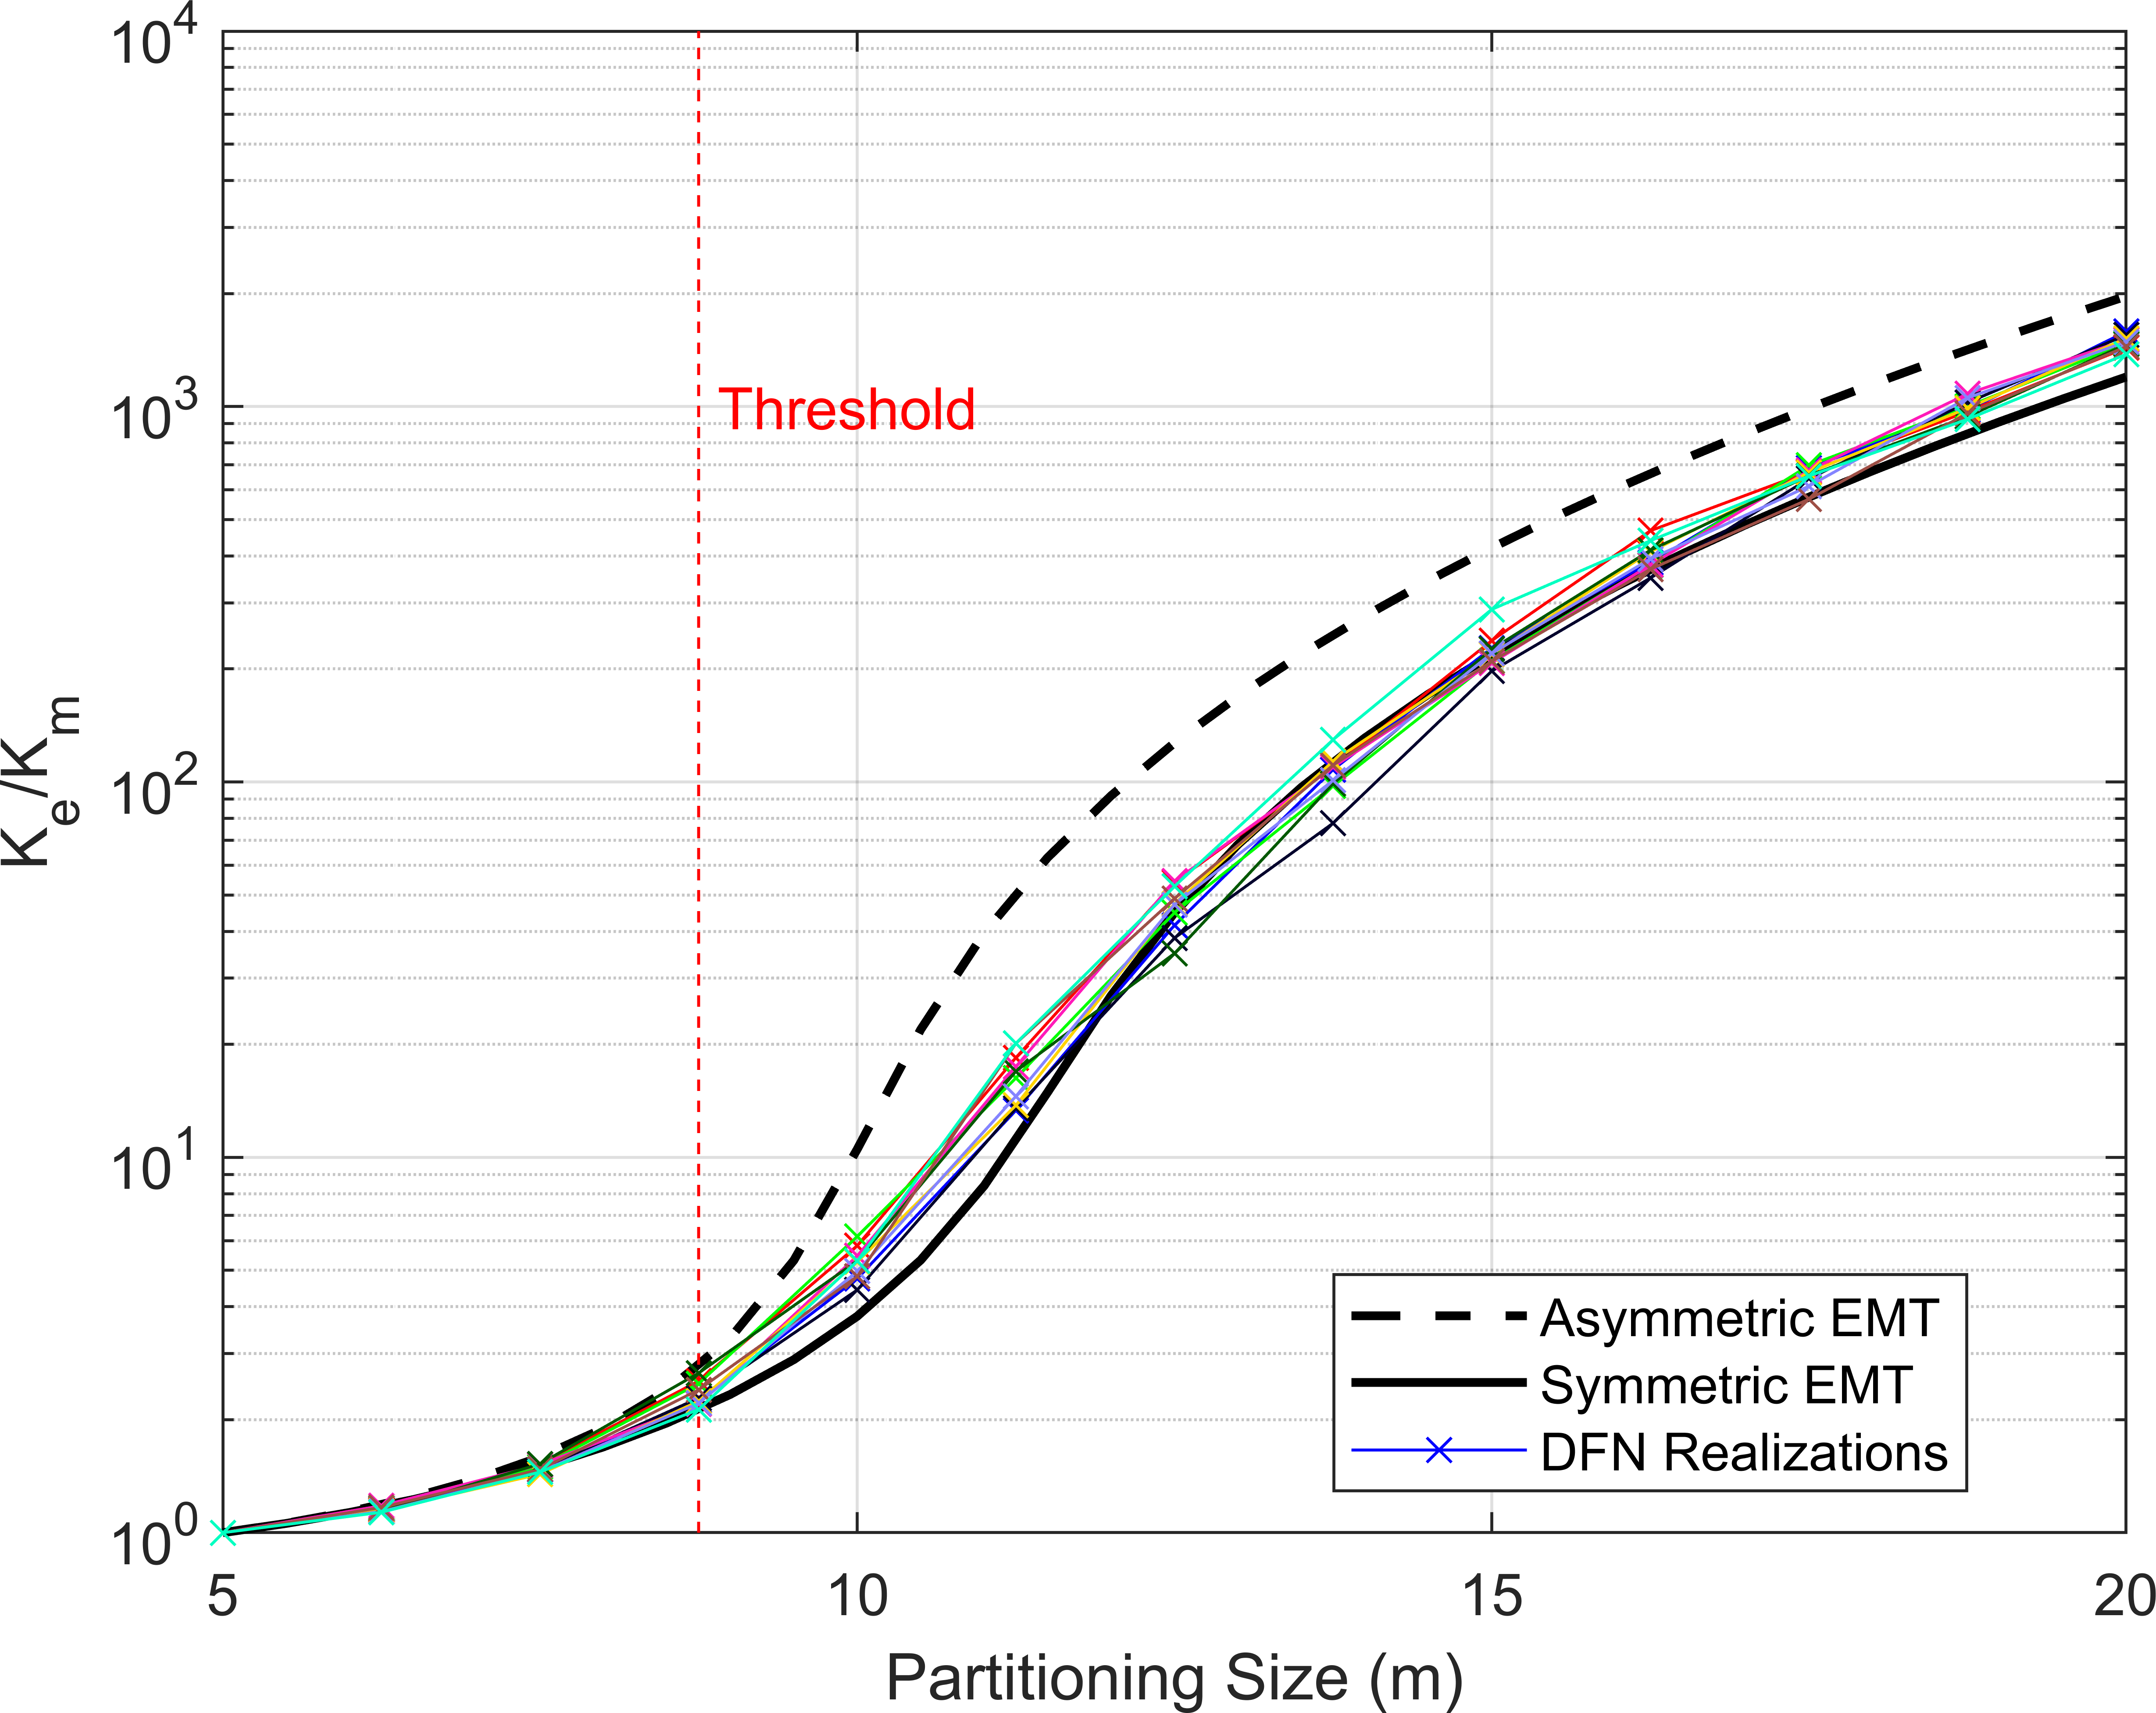
\includegraphics[width=\textwidth]{FSU/Plot_FSU_Case_01_nohead.png}
        \subcaption{Case 1}
        \label{fig:FSU_1}
    \end{subfigure}
    \begin{subfigure}{0.3\textwidth}
        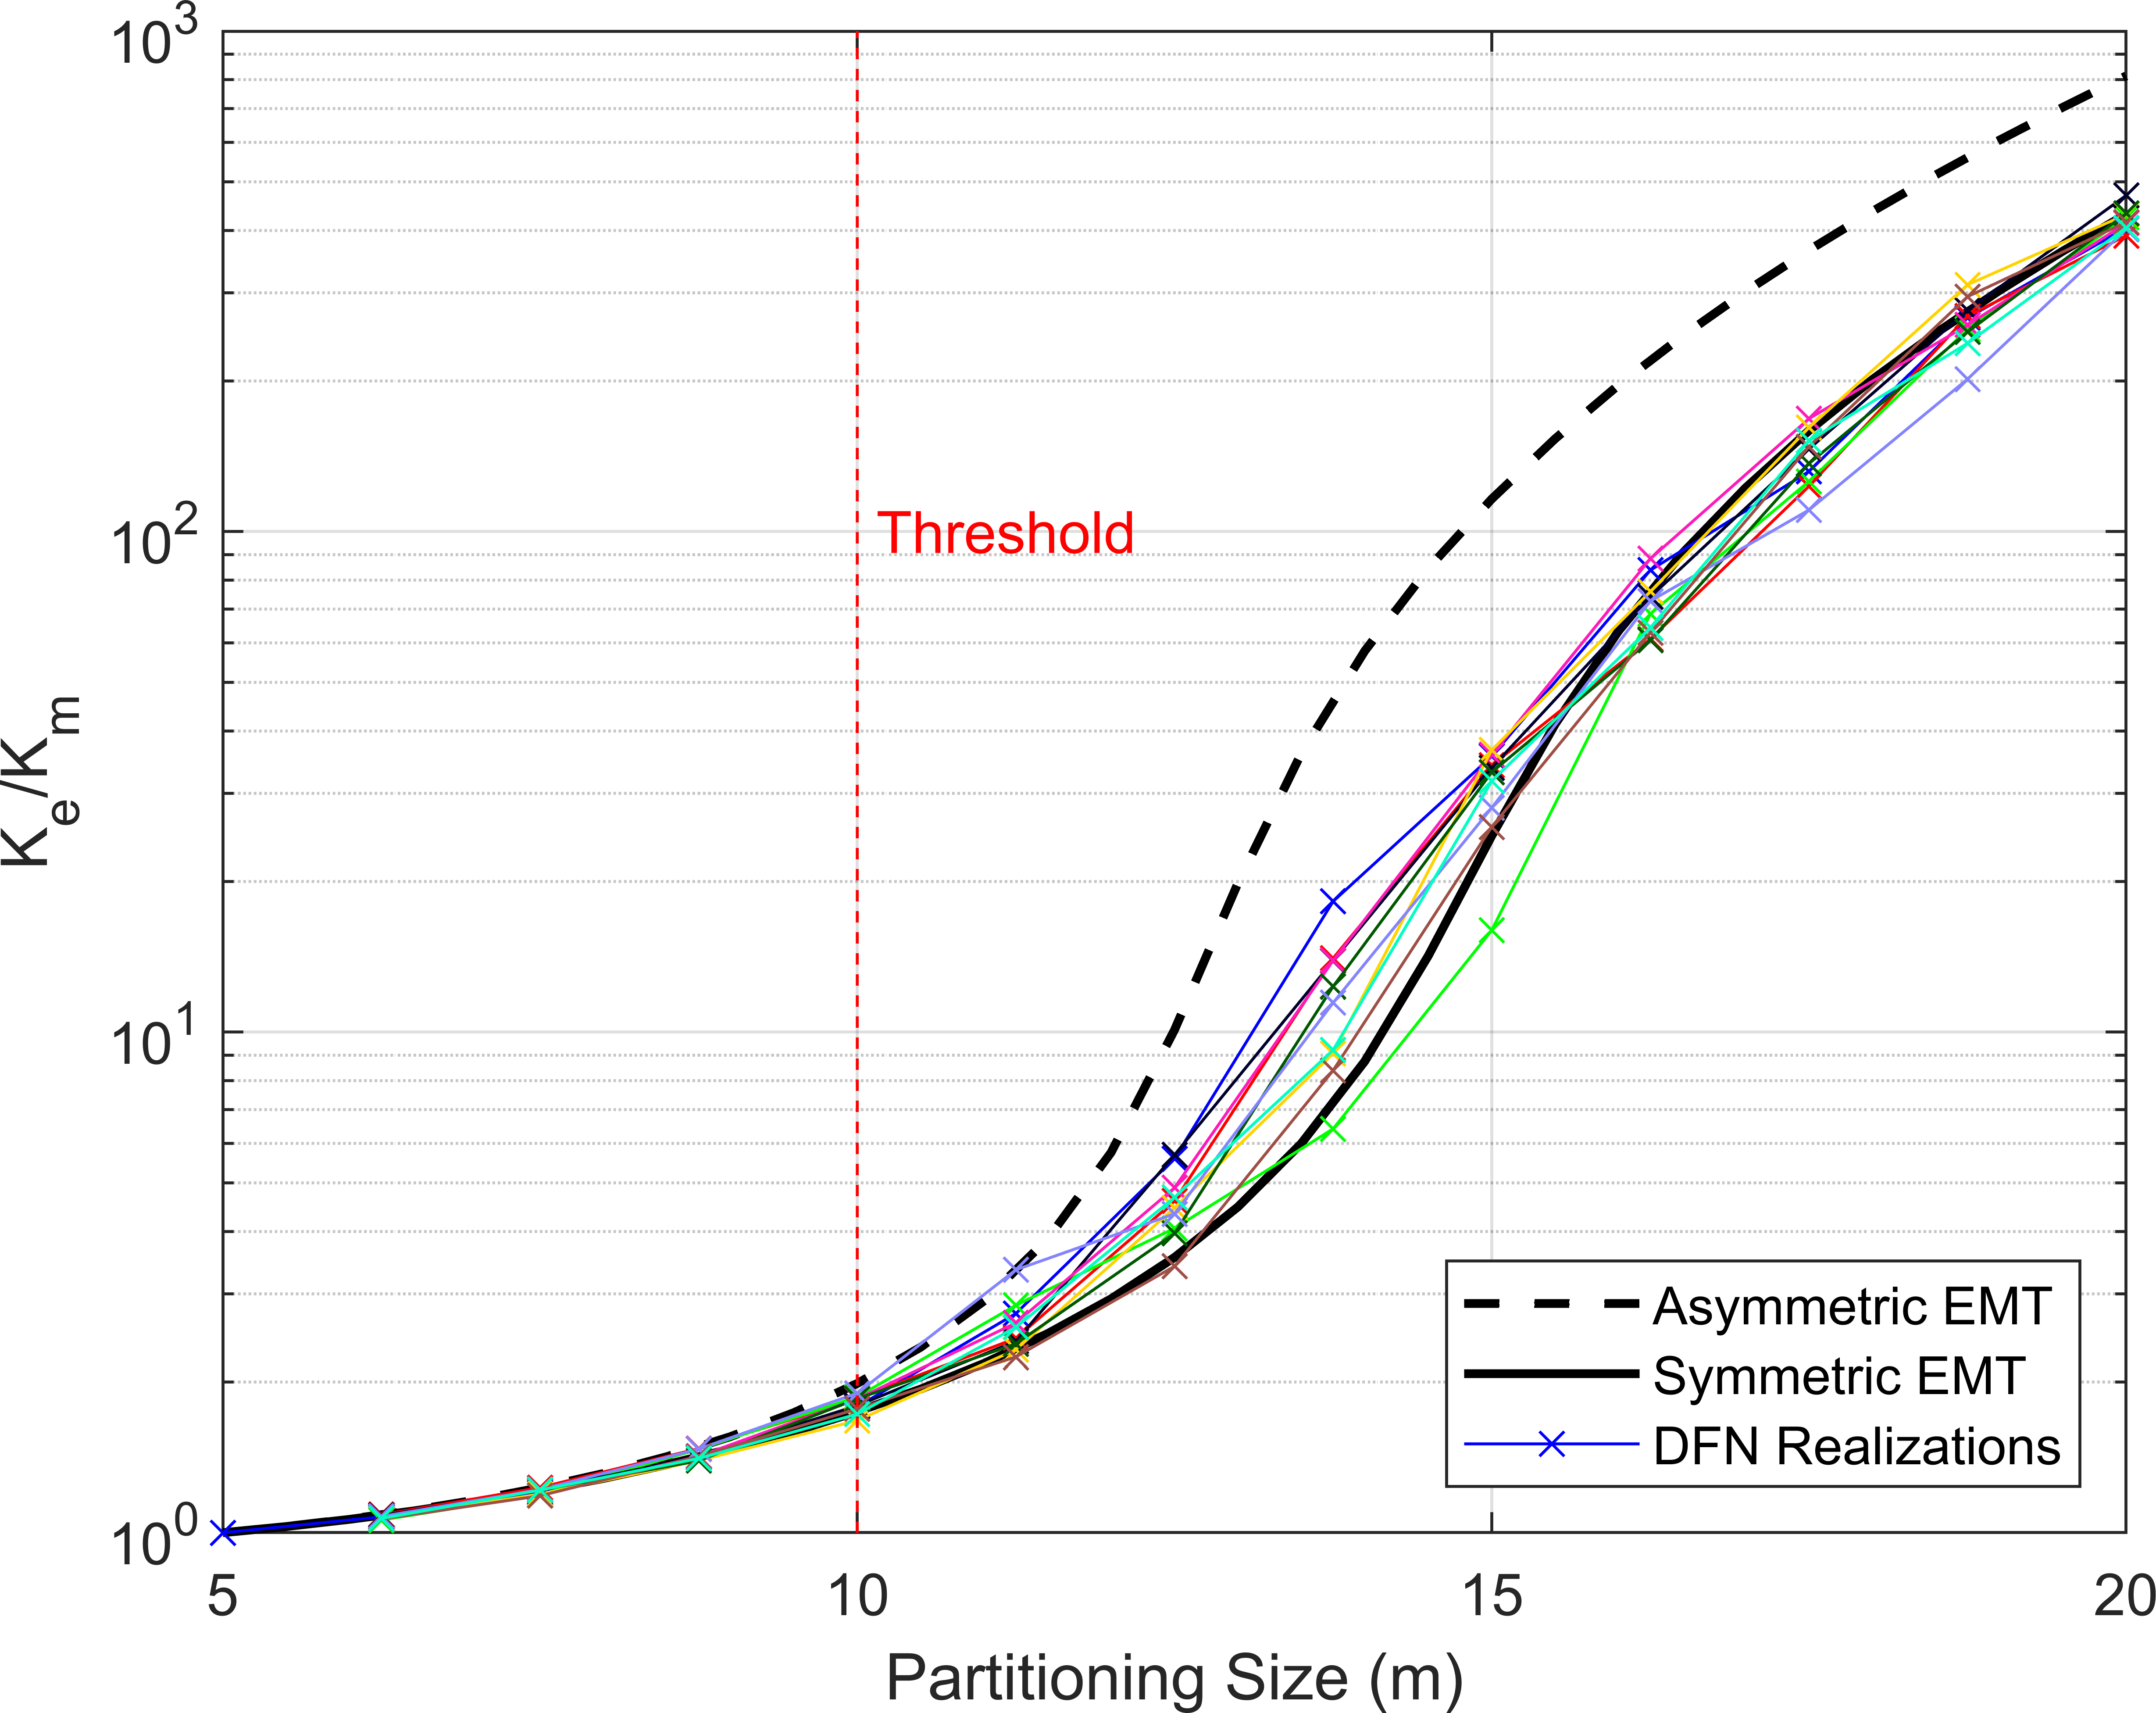
\includegraphics[width=\textwidth]{FSU/Plot_FSU_Case_02_nohead.png}
        \subcaption{Case 2}
        \label{fig:FSU_2}
    \end{subfigure}
    \begin{subfigure}{0.3\textwidth}
        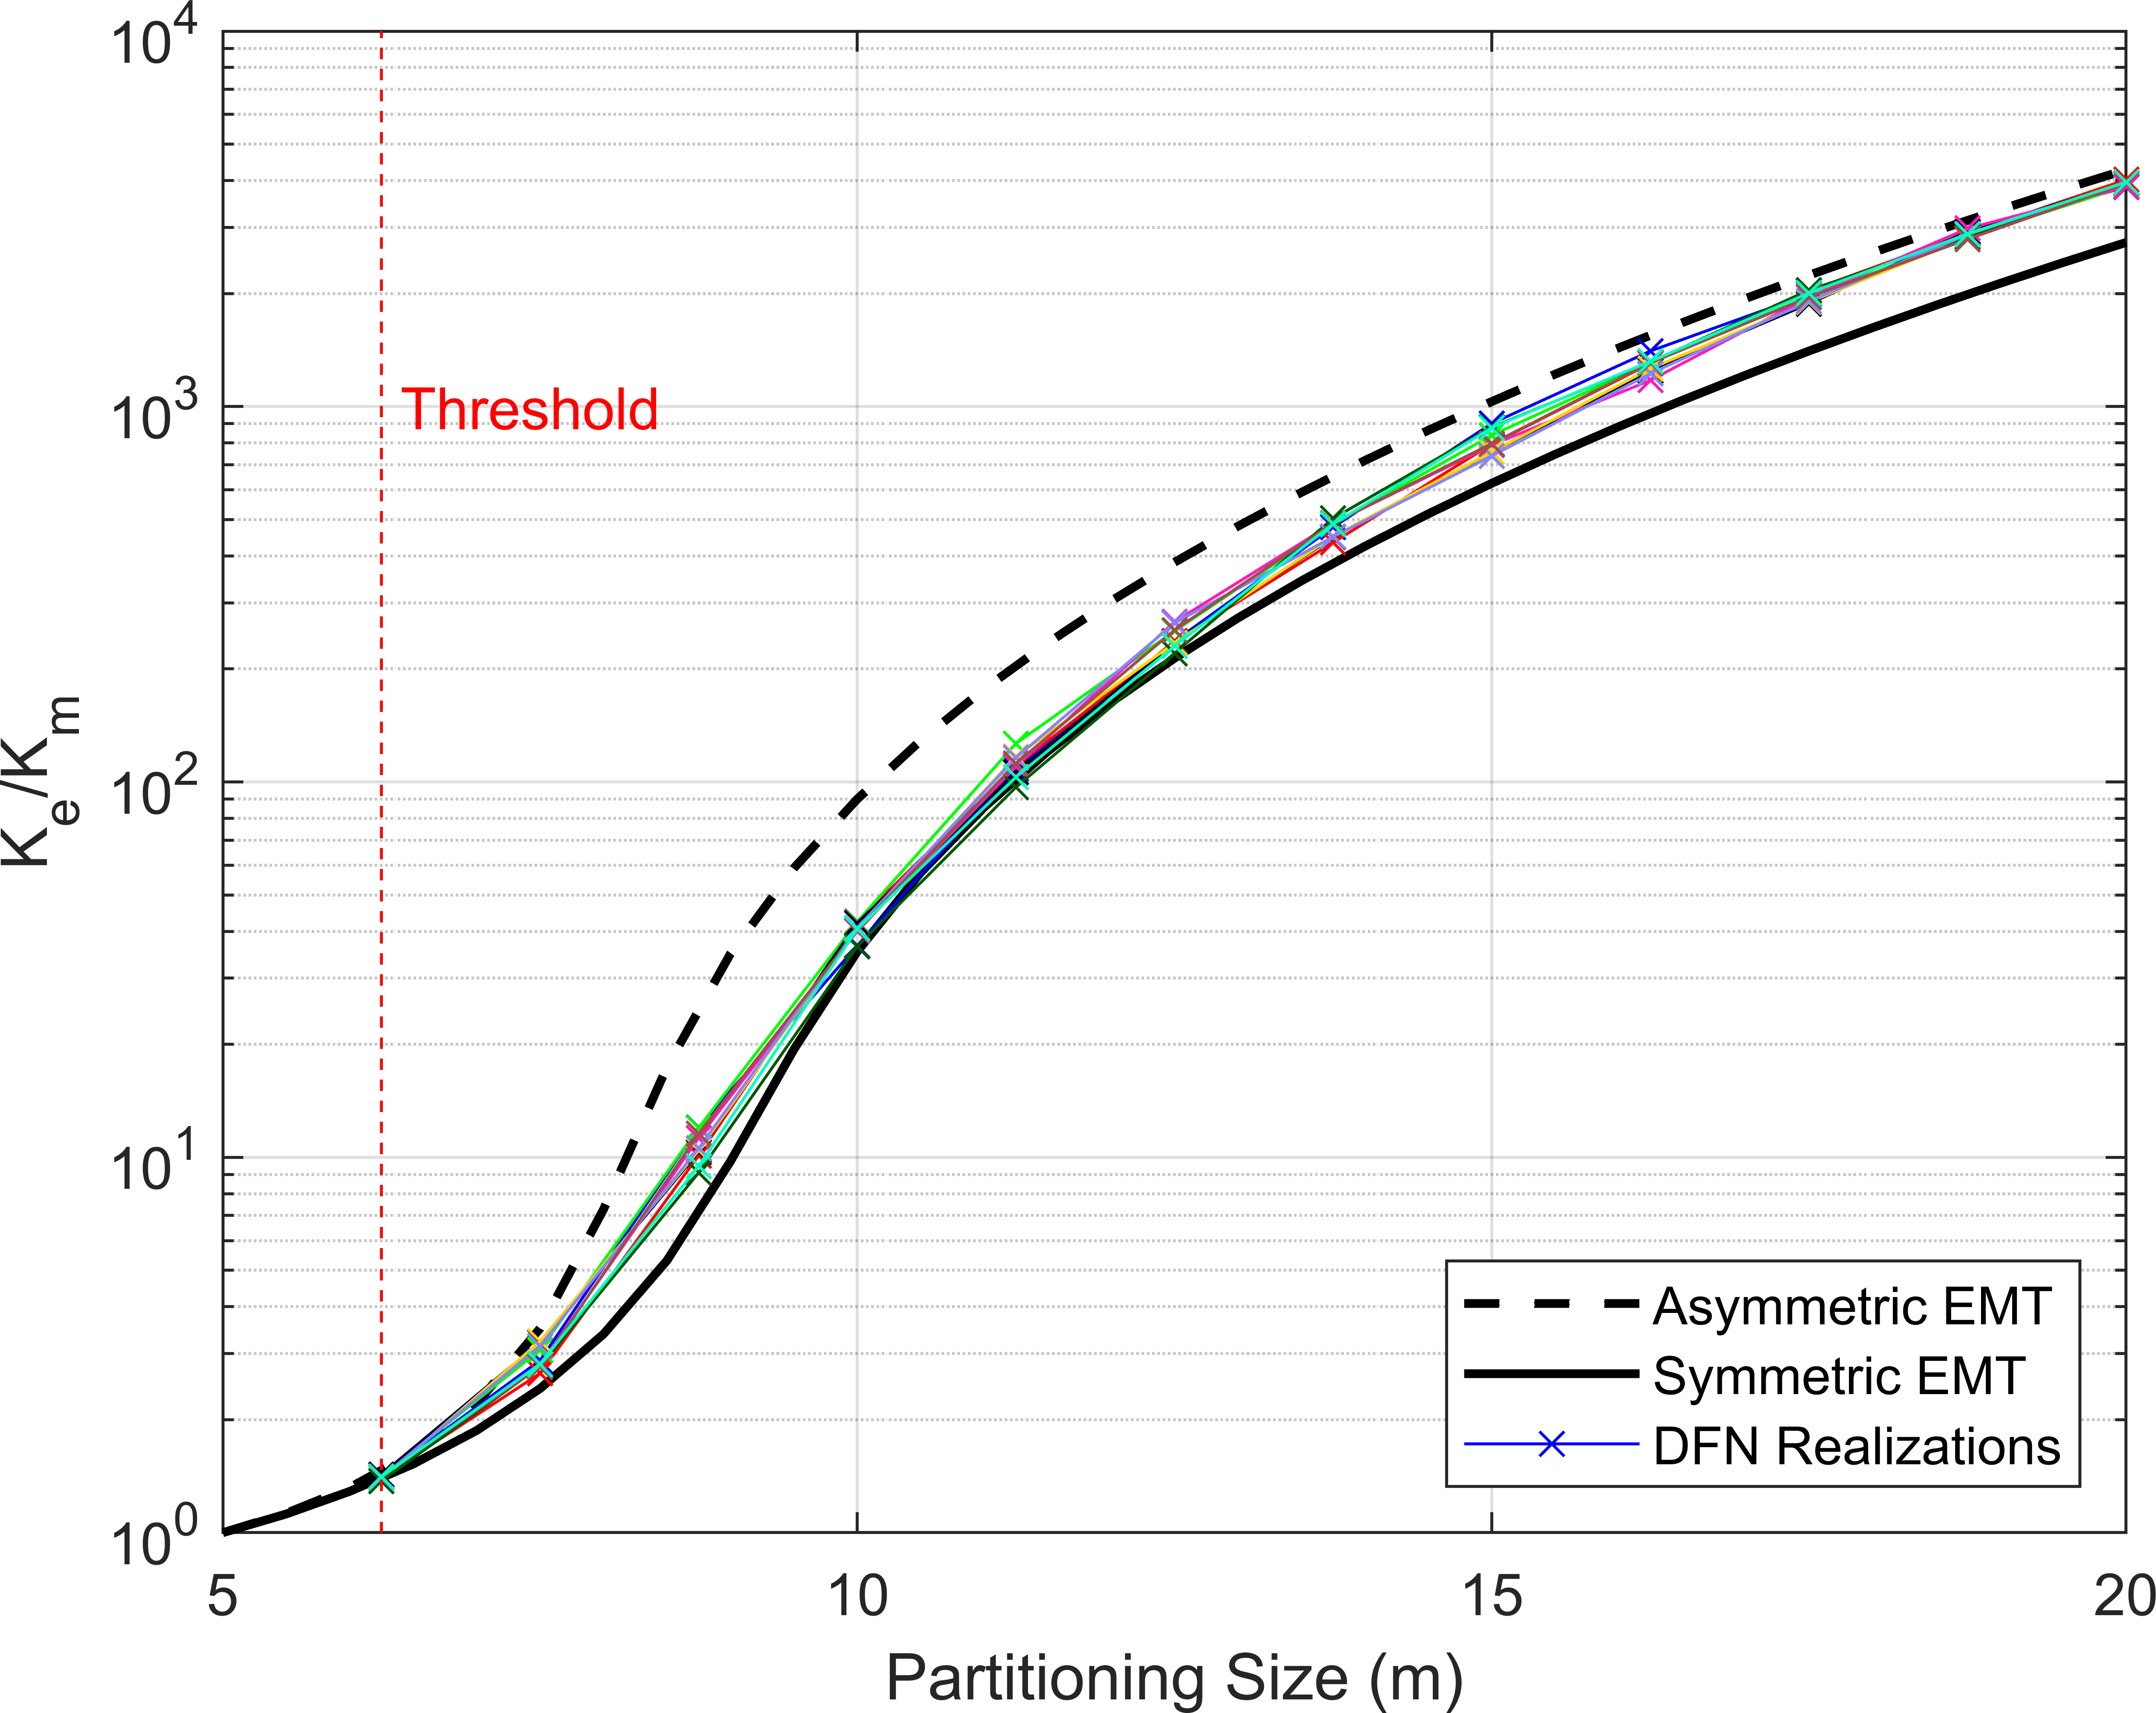
\includegraphics[width=\textwidth]{FSU/Plot_FSU_Case_03_nohead.png}
        \subcaption{Case 3}
        \label{fig:FSU_3}
    \end{subfigure}
    \\
    \begin{subfigure}{0.3\textwidth}
        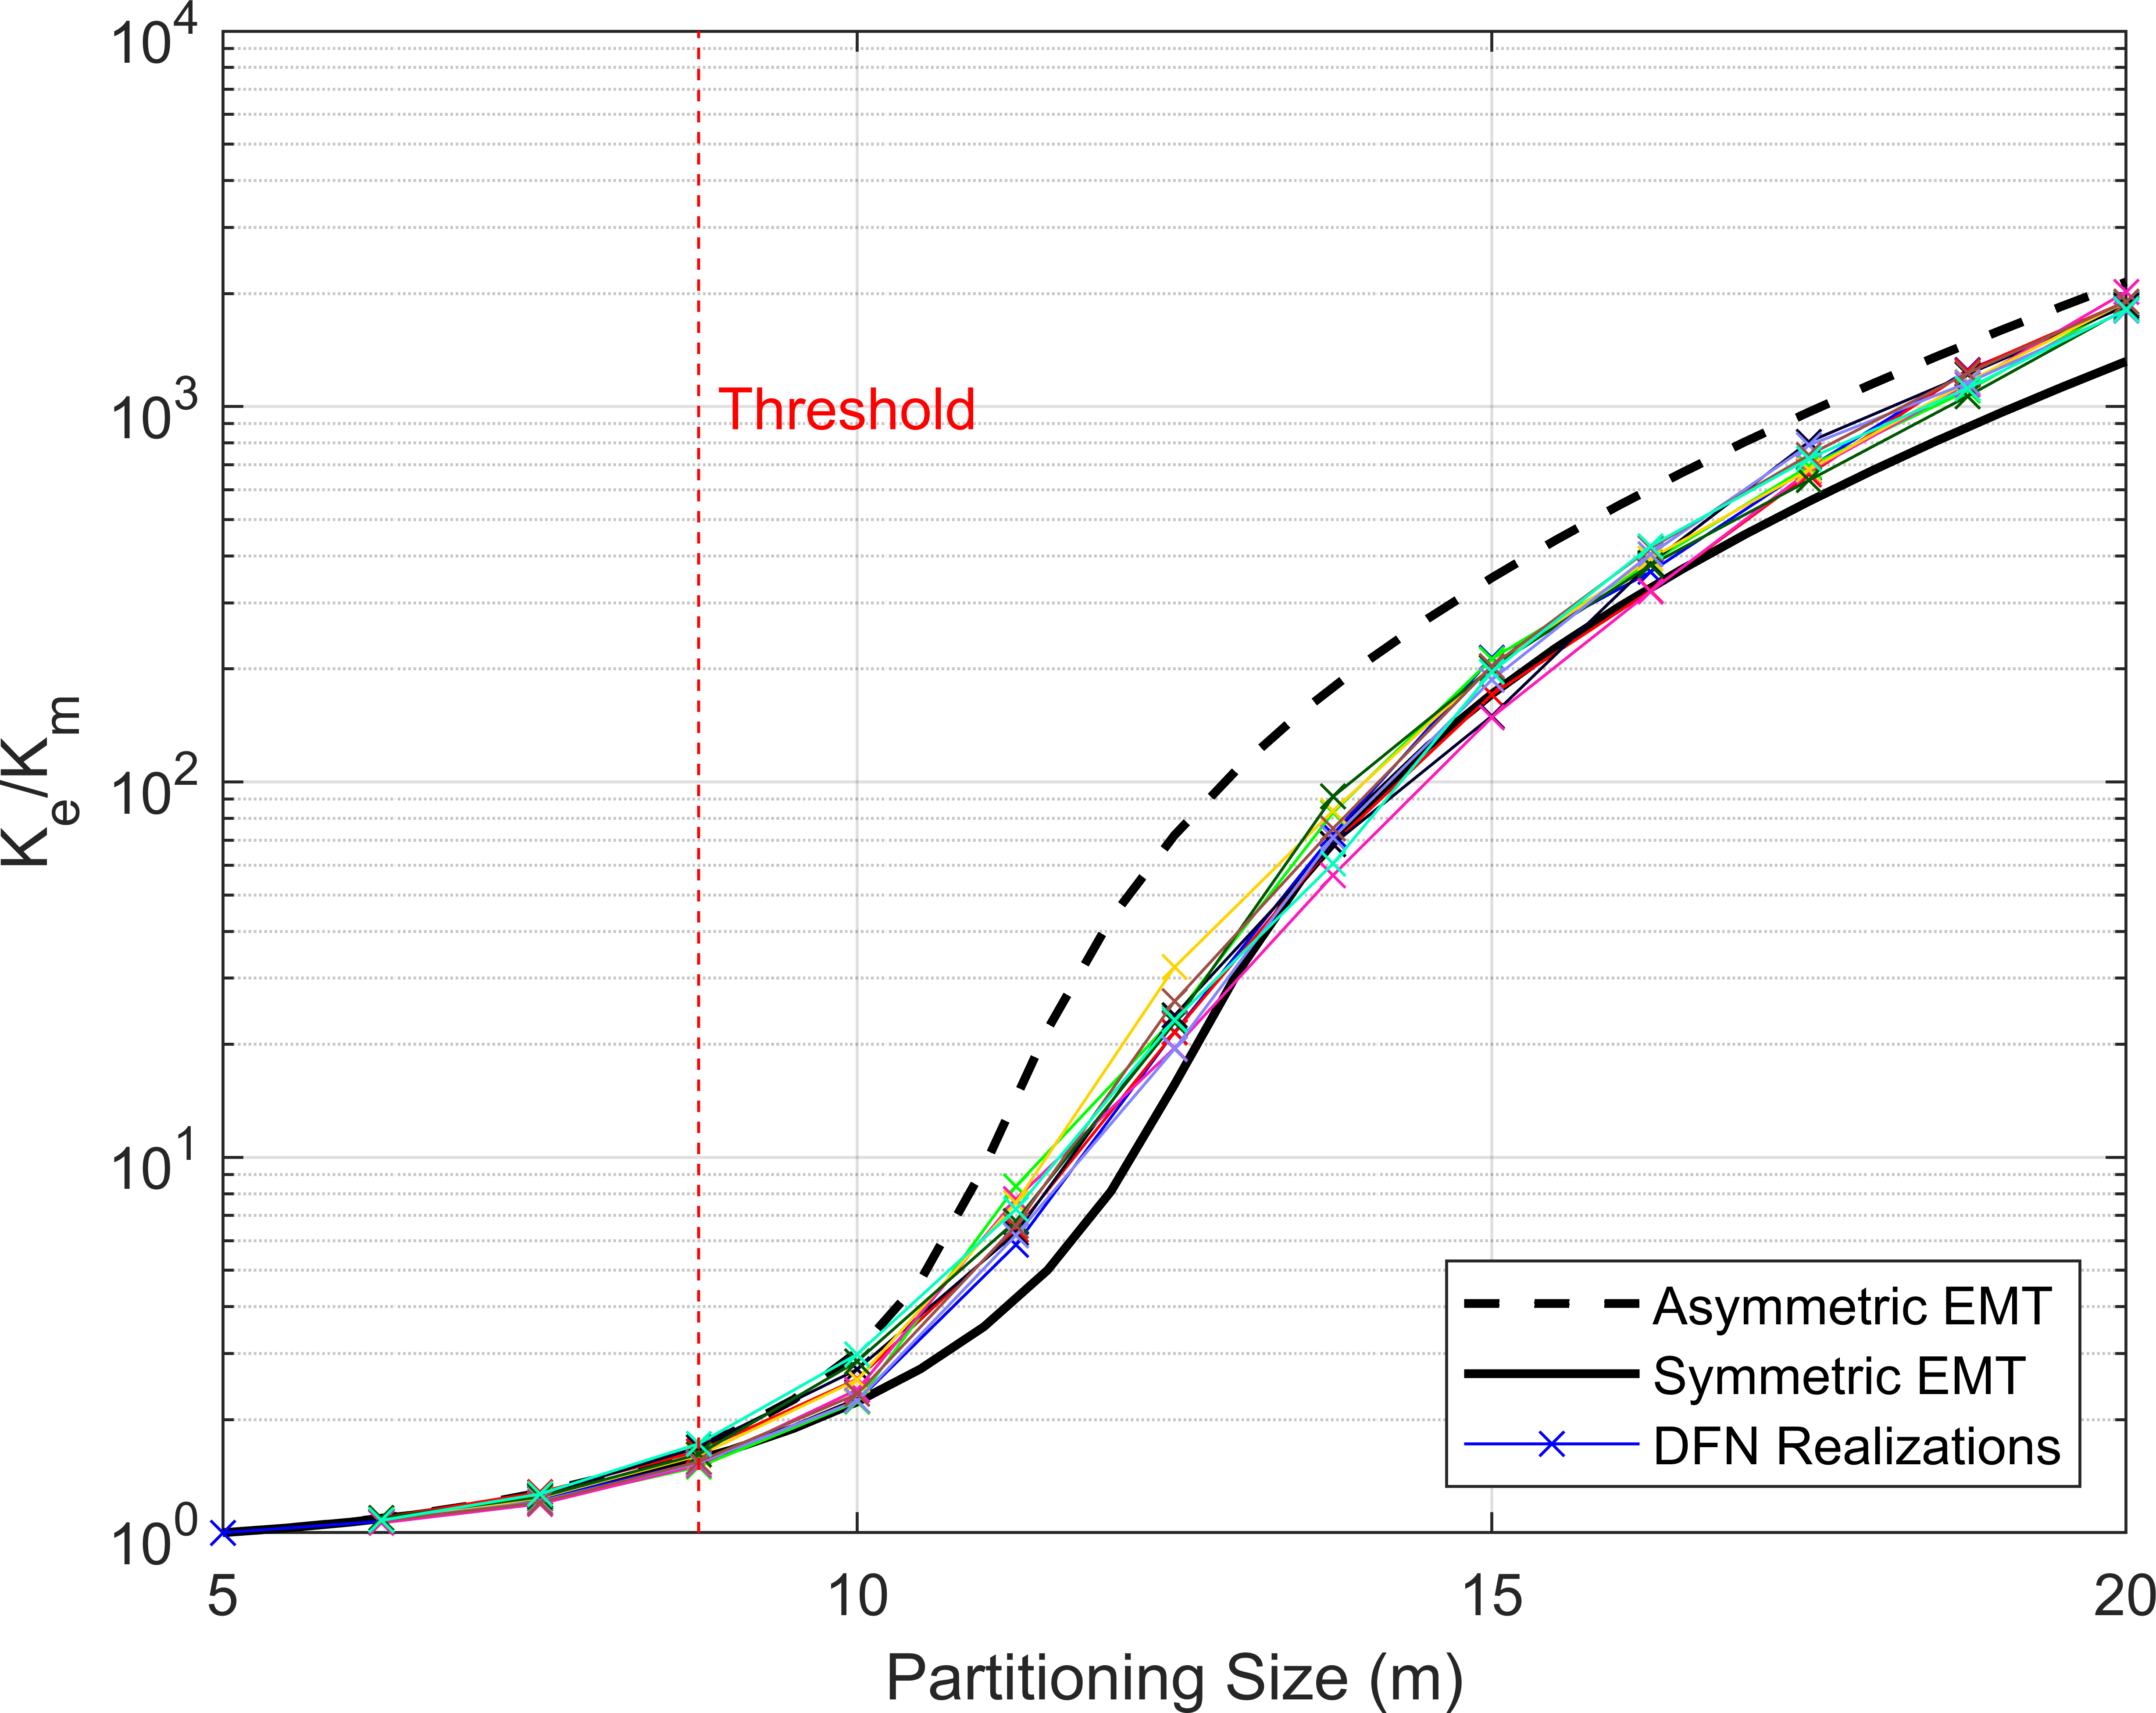
\includegraphics[width=\textwidth]{FSU/Plot_FSU_Case_04_nohead.png}
        \subcaption{Case 4}
        \label{fig:FSU_4}
    \end{subfigure}
    \begin{subfigure}{0.3\textwidth}
        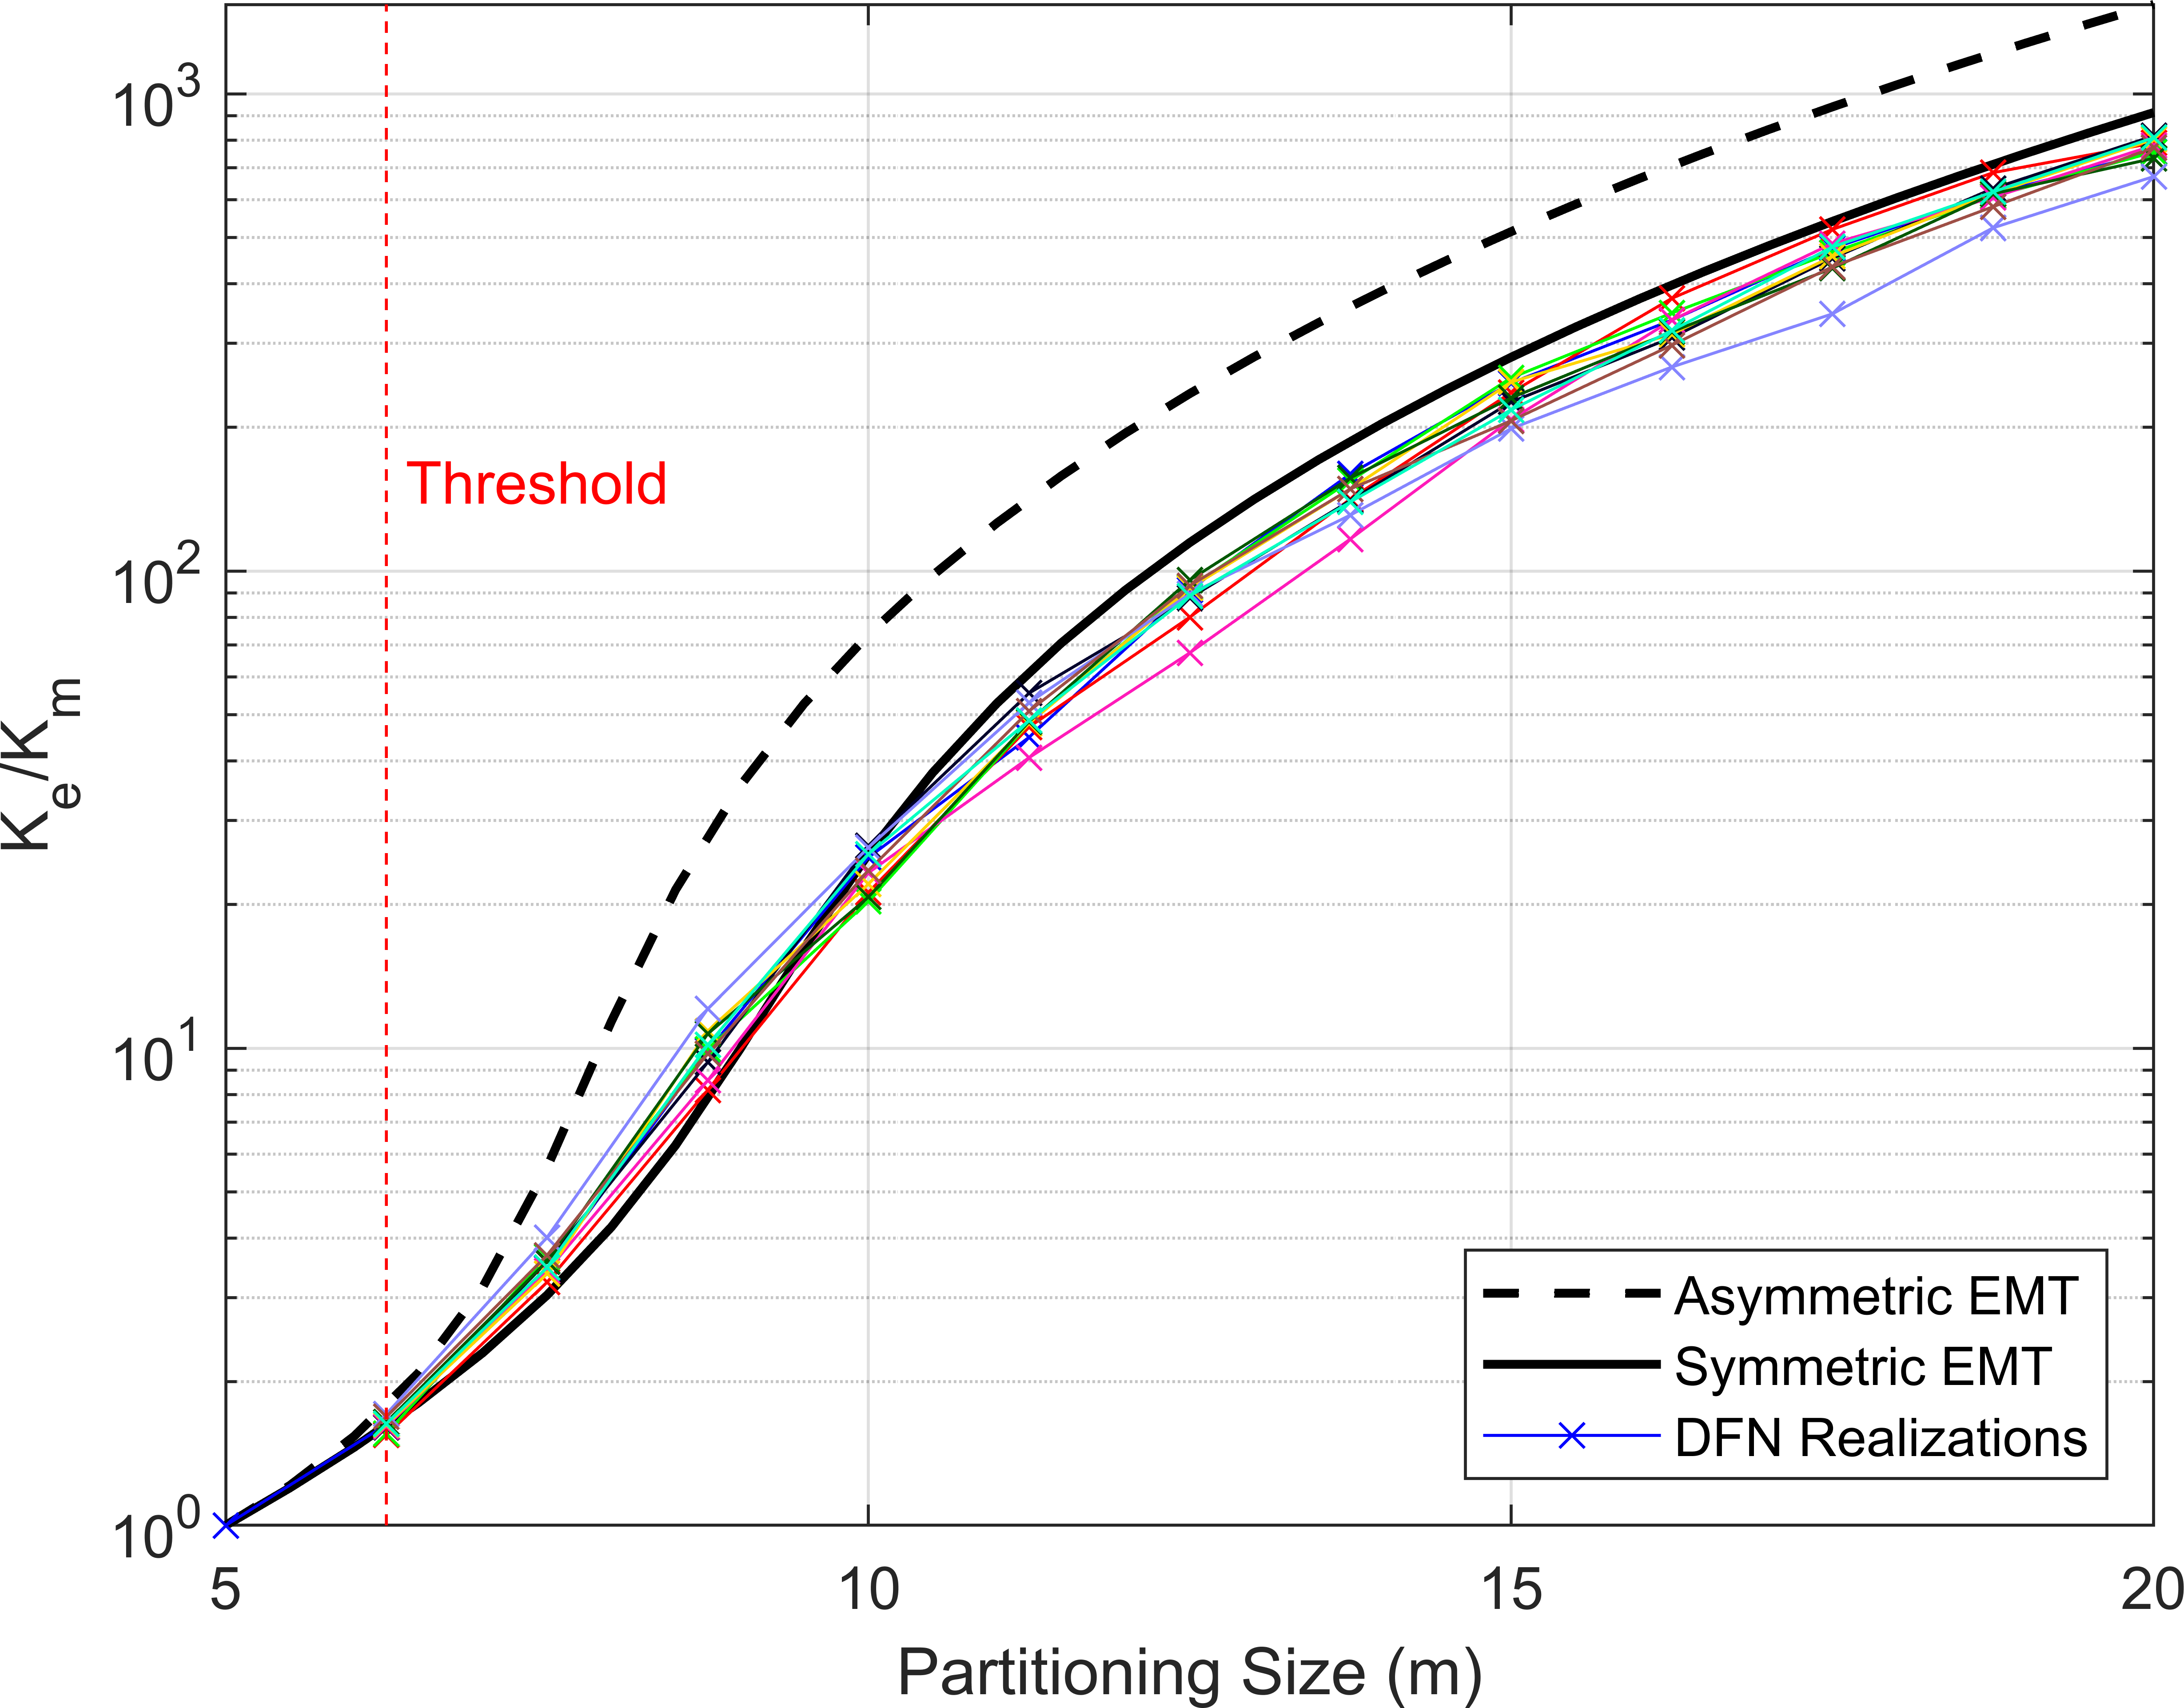
\includegraphics[width=\textwidth]{FSU/Plot_FSU_Case_05_nohead.png}
        \subcaption{Case 5}
        \label{fig:FSU_5}
    \end{subfigure}
    \begin{subfigure}{0.3\textwidth}
        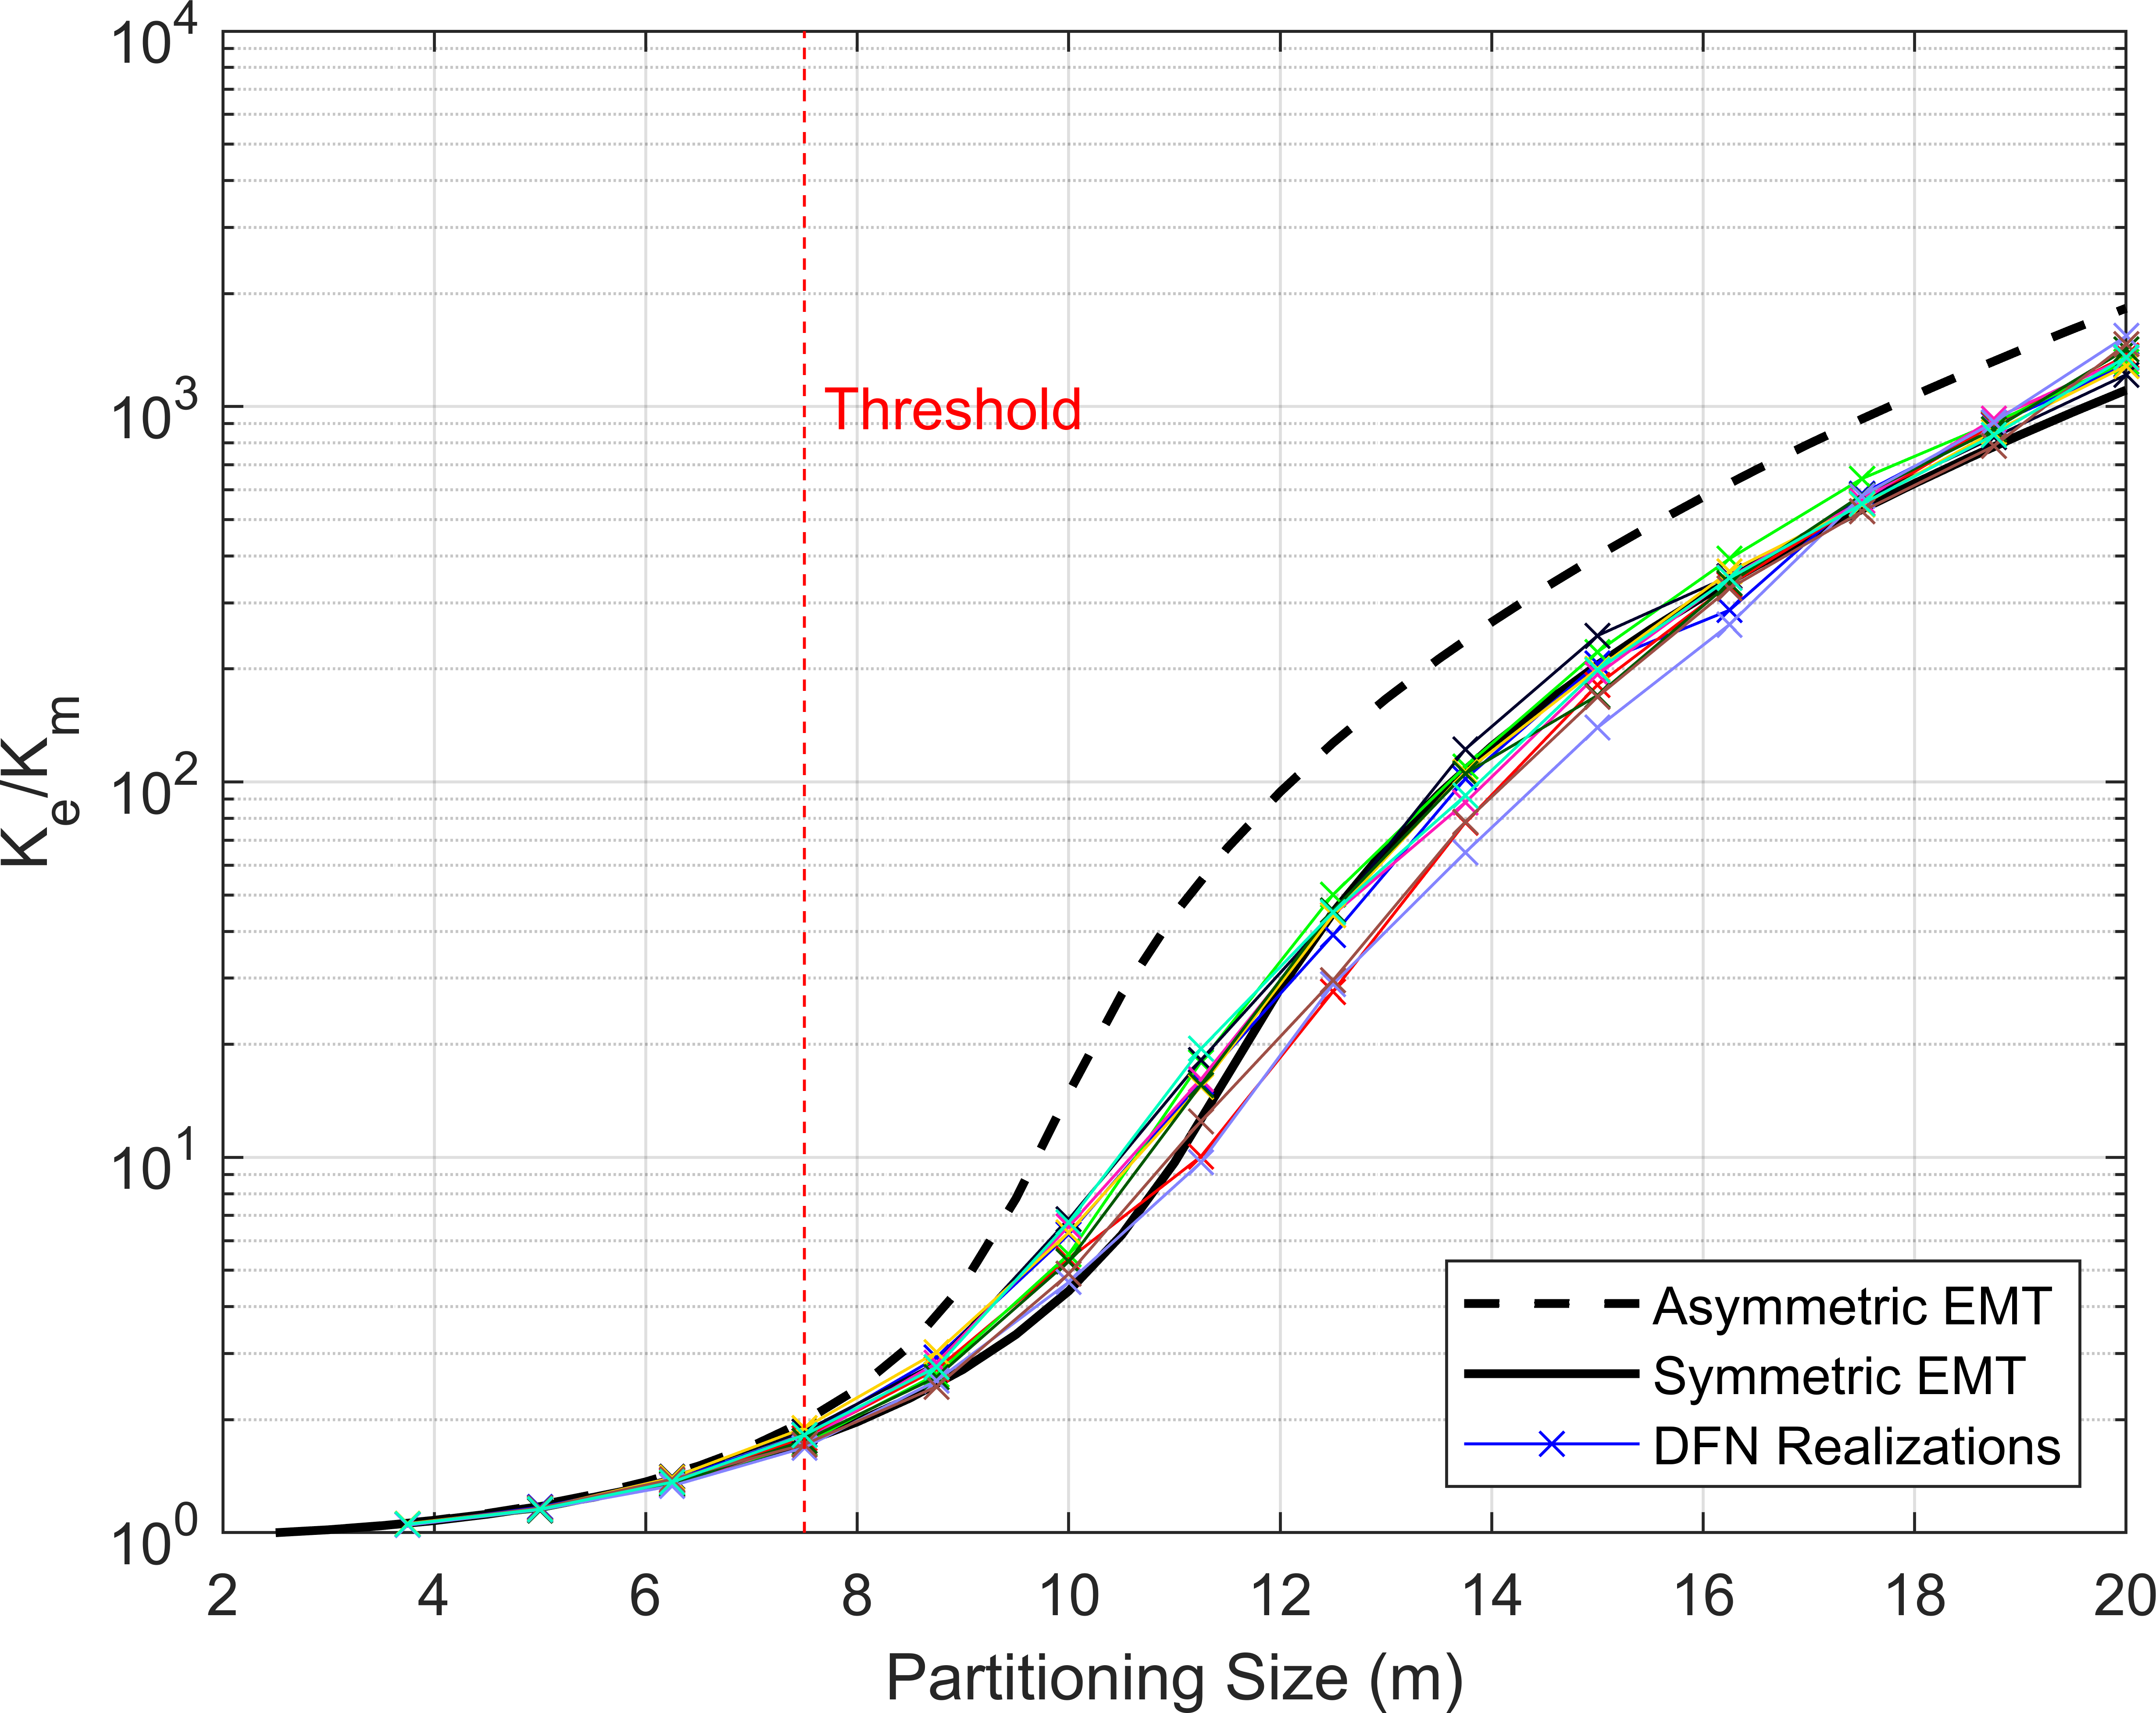
\includegraphics[width=\textwidth]{FSU/Plot_FSU_Case_06_nohead.png}
        \subcaption{Case 6}
        \label{fig:FSU_6}
    \end{subfigure}
    \\
    \begin{subfigure}{0.3\textwidth}
        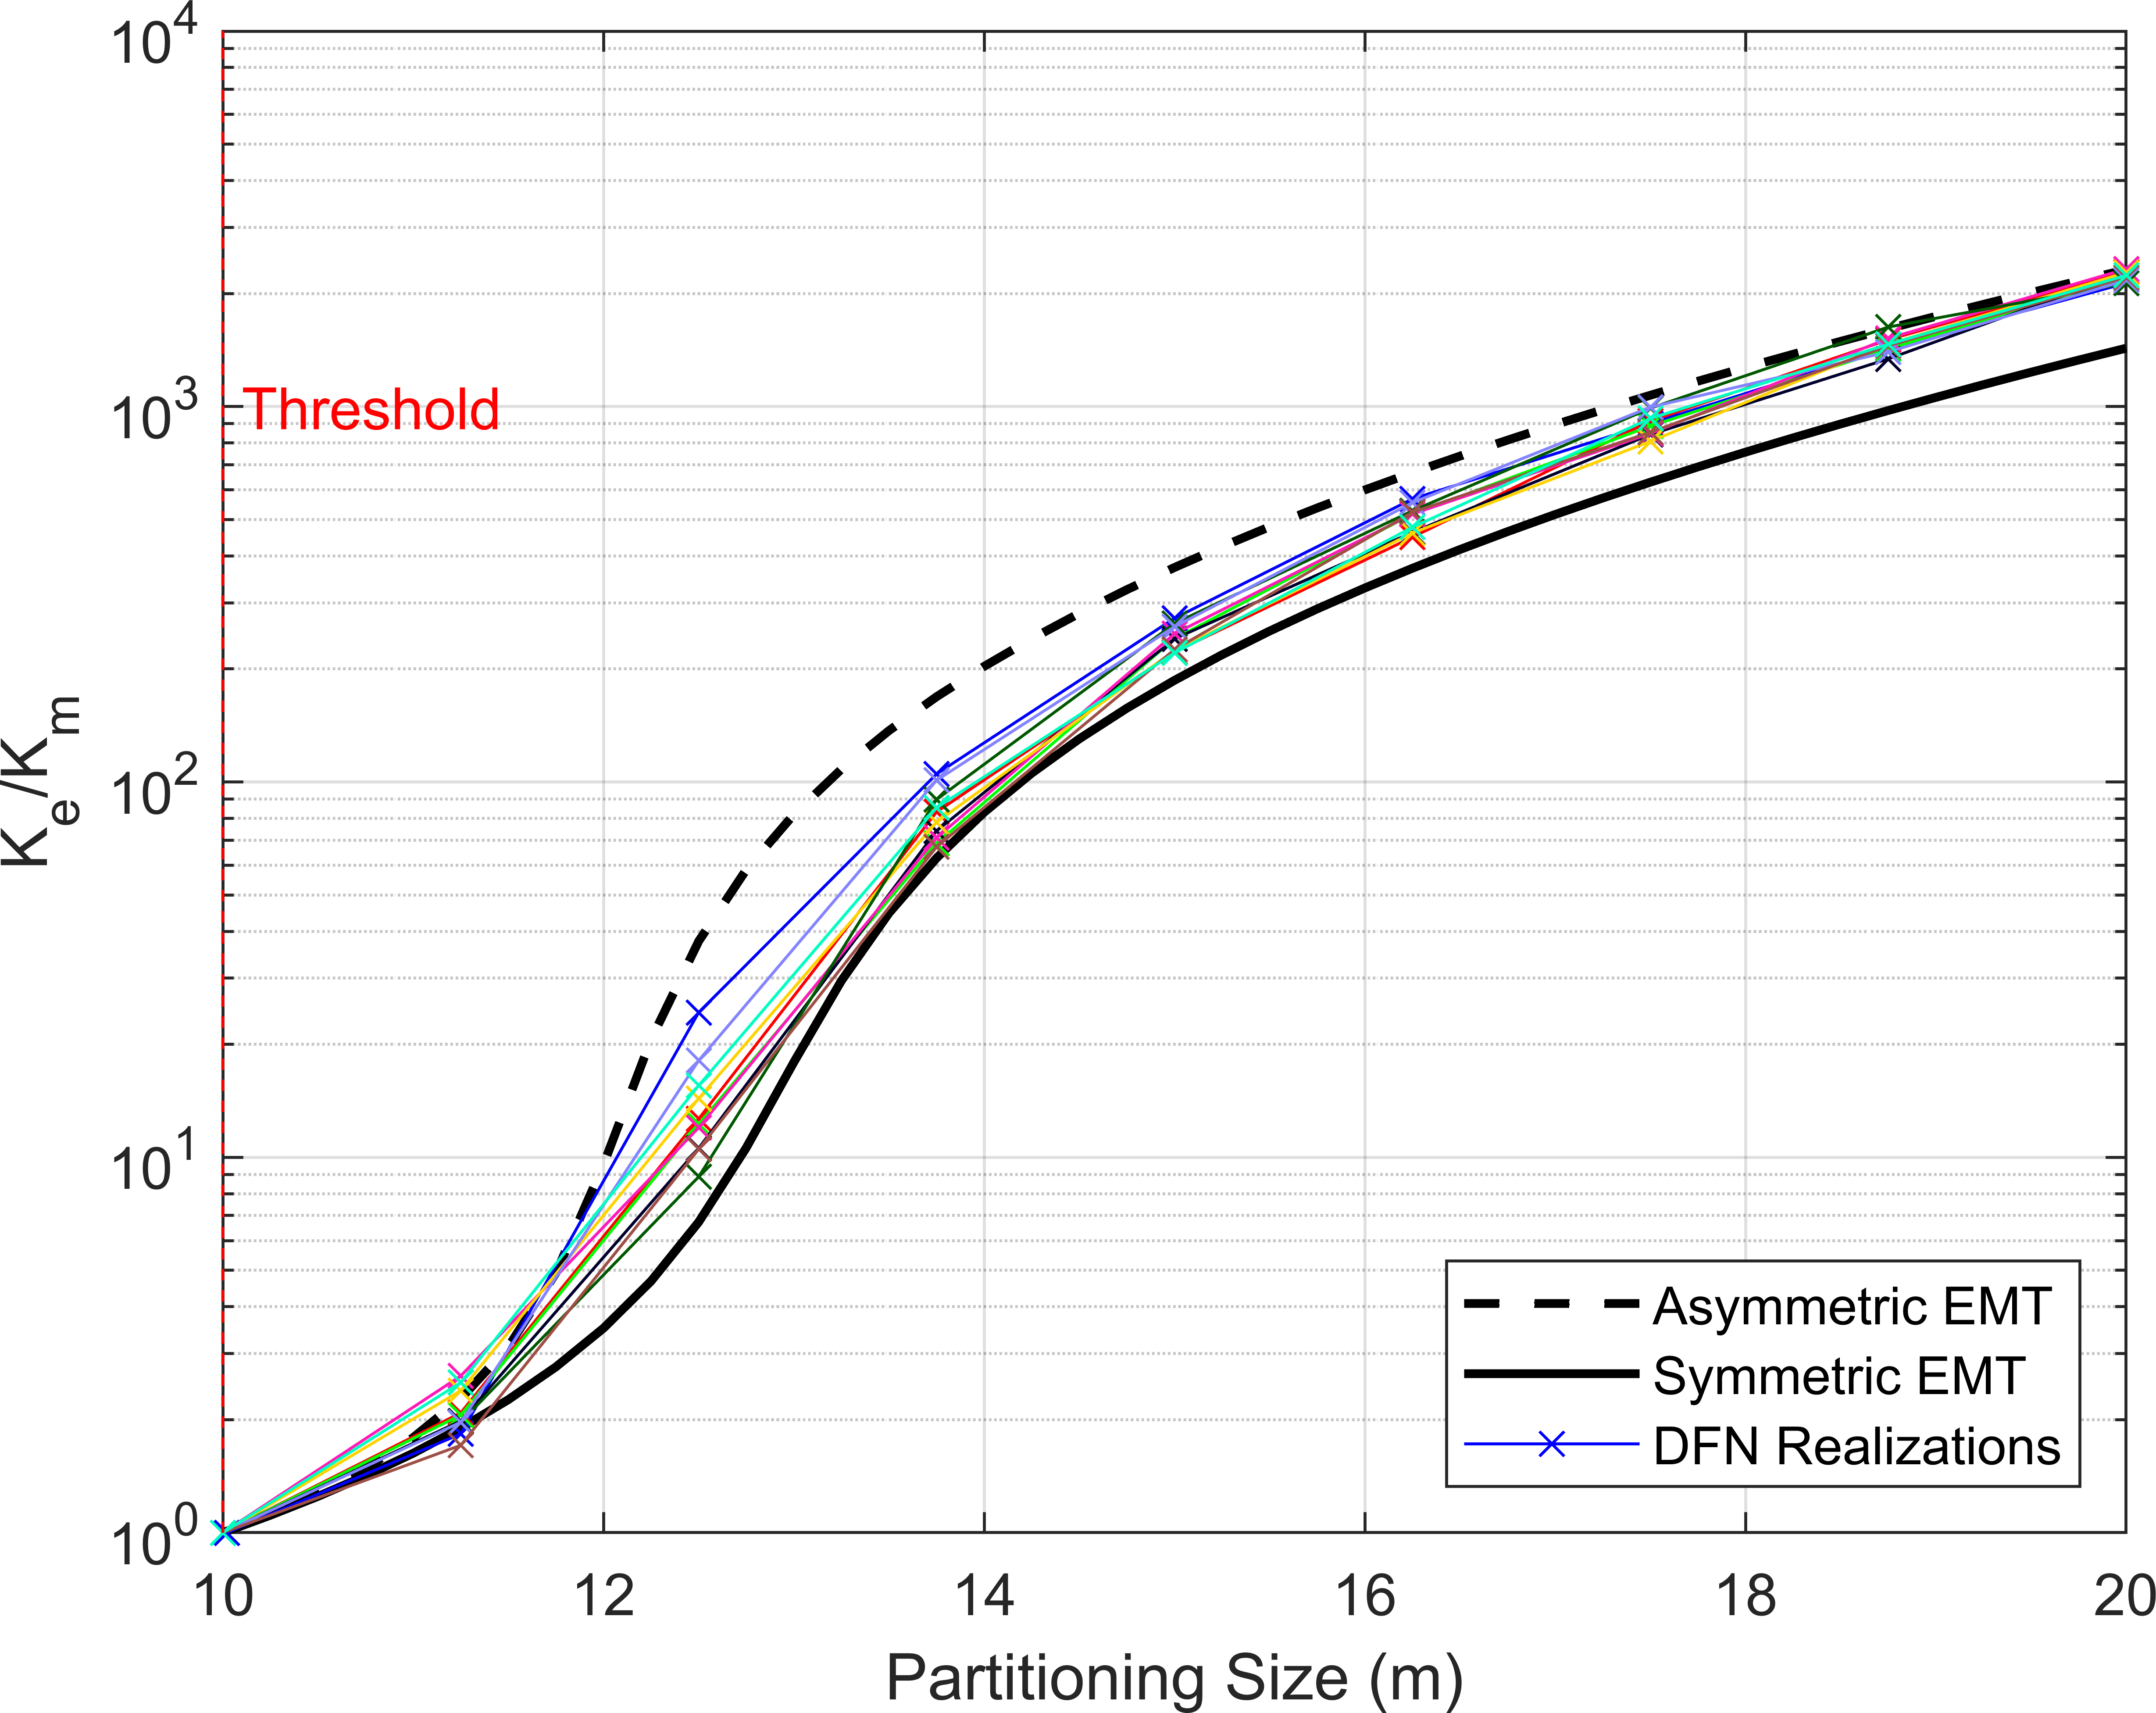
\includegraphics[width=\textwidth]{FSU/Plot_FSU_Case_07_nohead.png}
        \subcaption{Case 7}
        \label{fig:FSU_7}
    \end{subfigure}
    \begin{subfigure}{0.3\textwidth}
        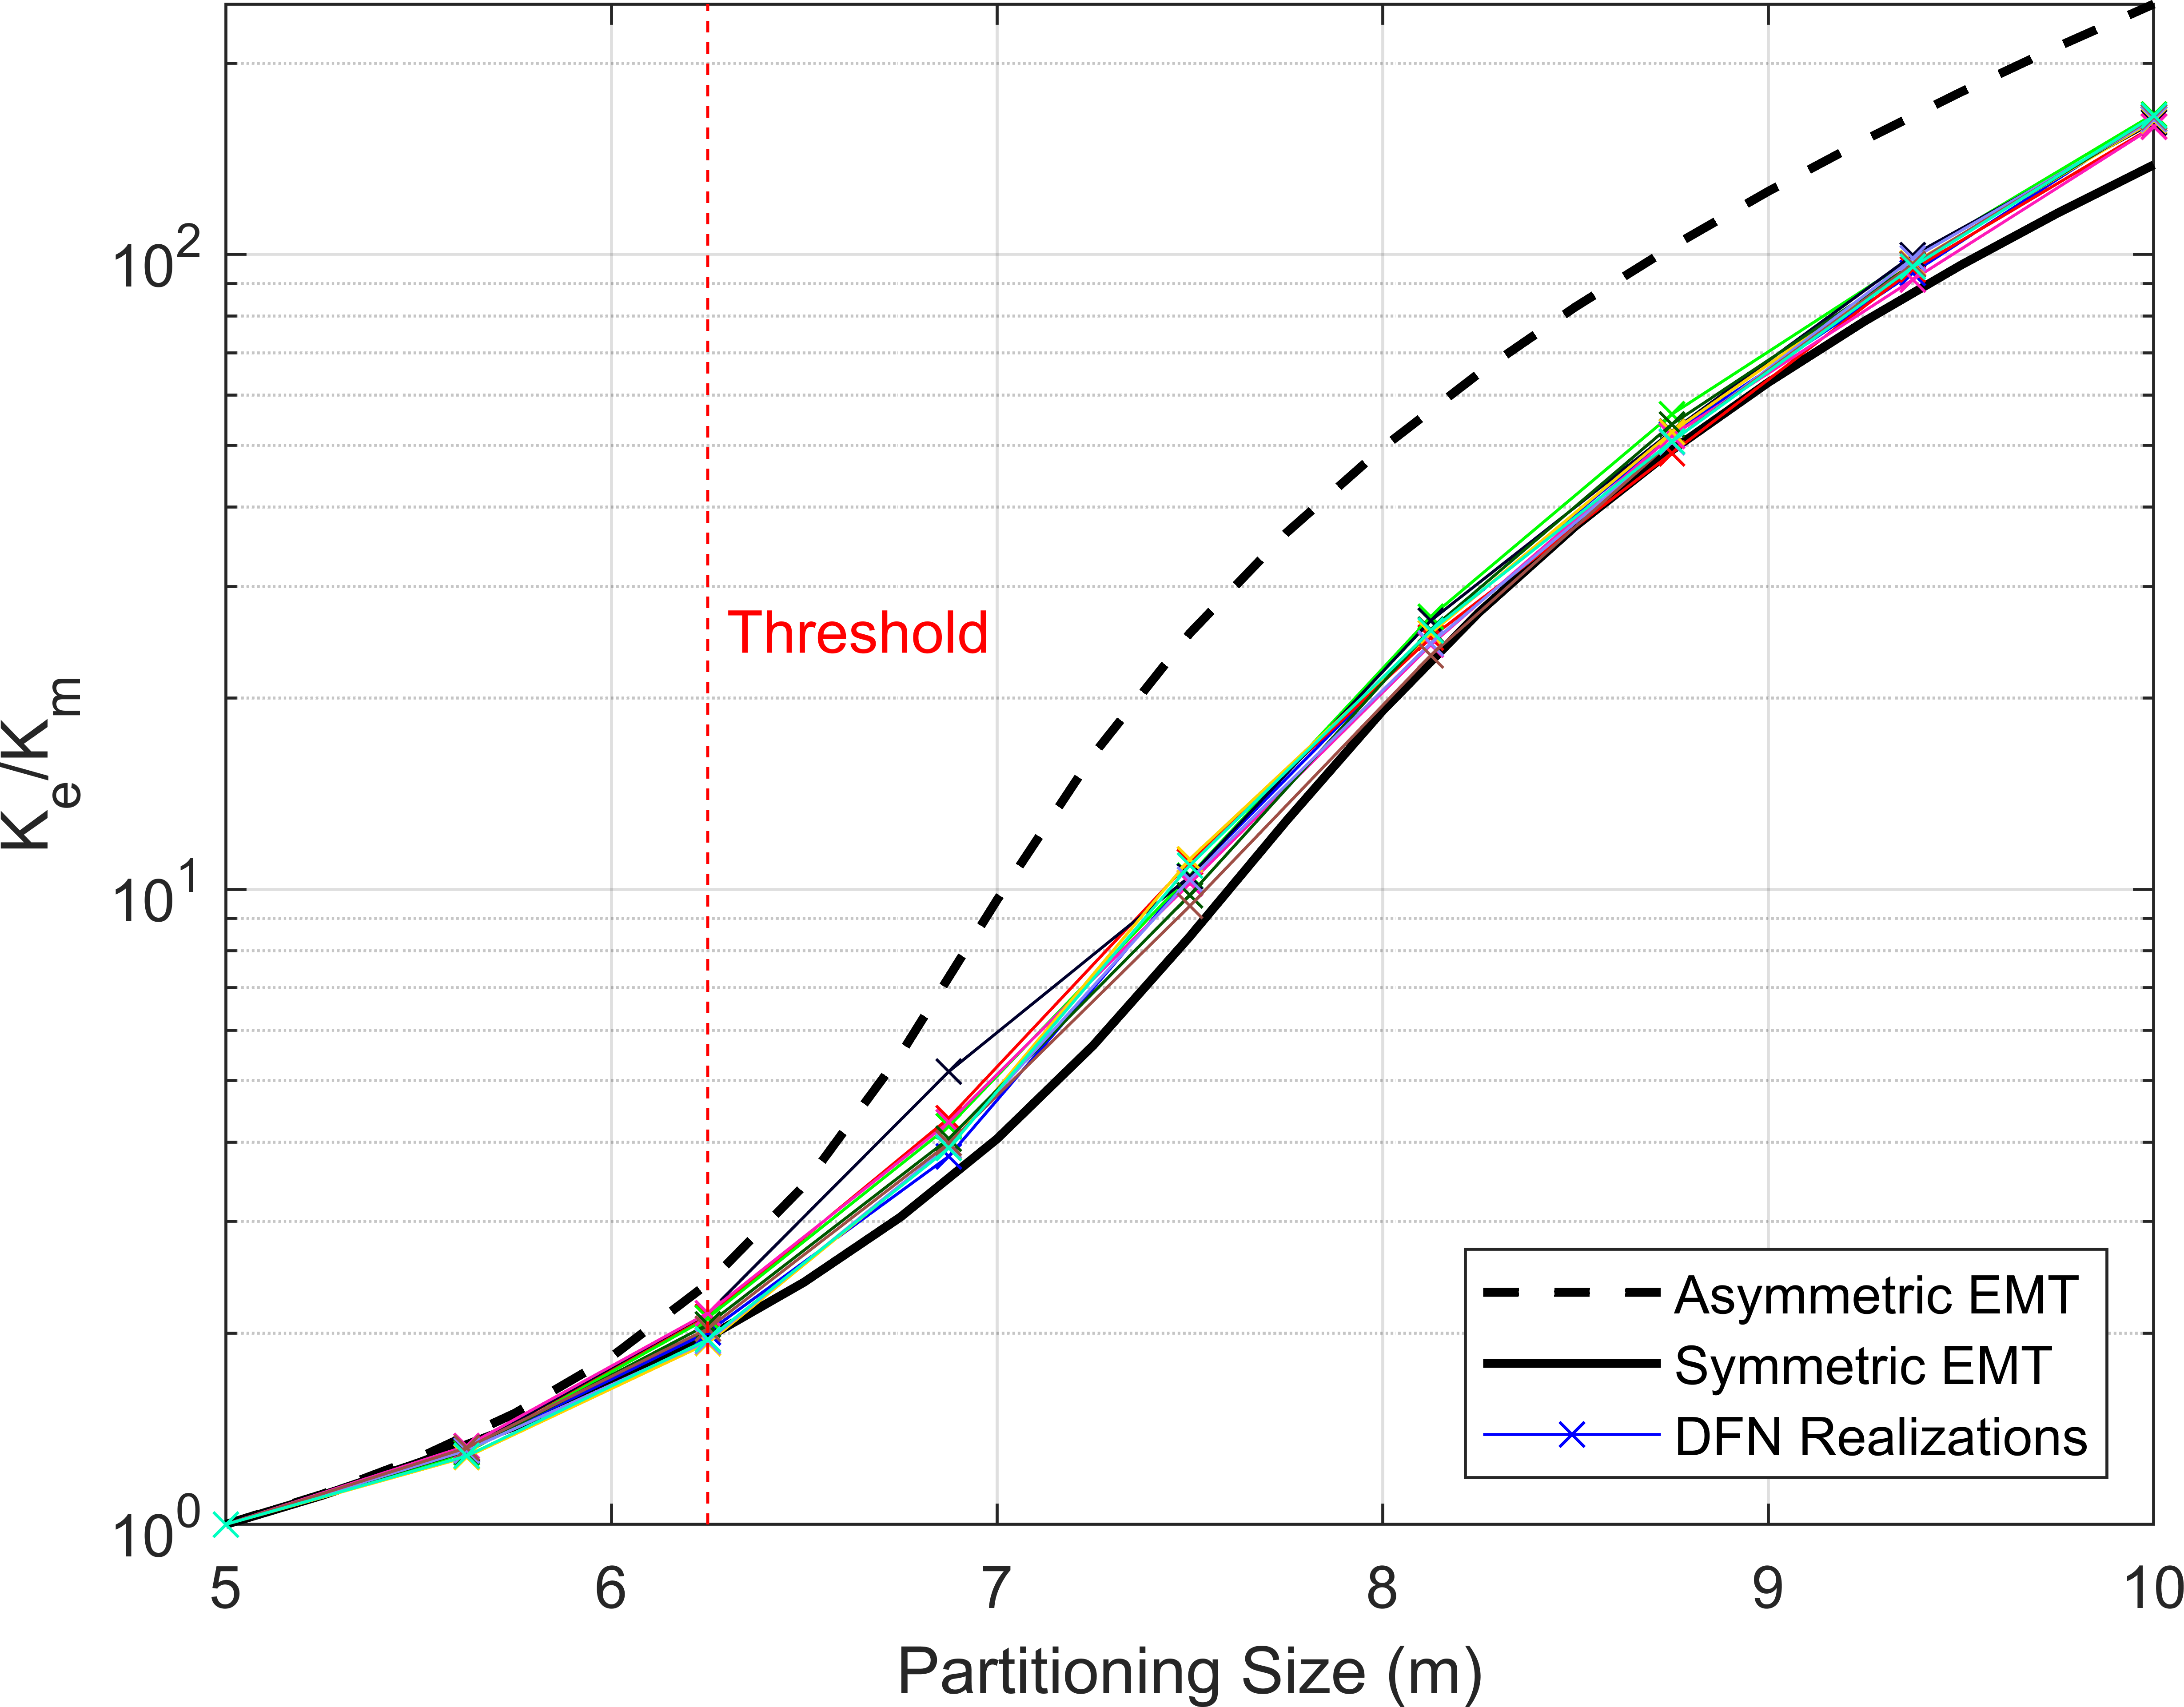
\includegraphics[width=\textwidth]{FSU/Plot_FSU_Case_08_nohead.png}
        \subcaption{Case 8}
        \label{fig:FSU_8}
    \end{subfigure}
    \begin{subfigure}{0.3\textwidth}
        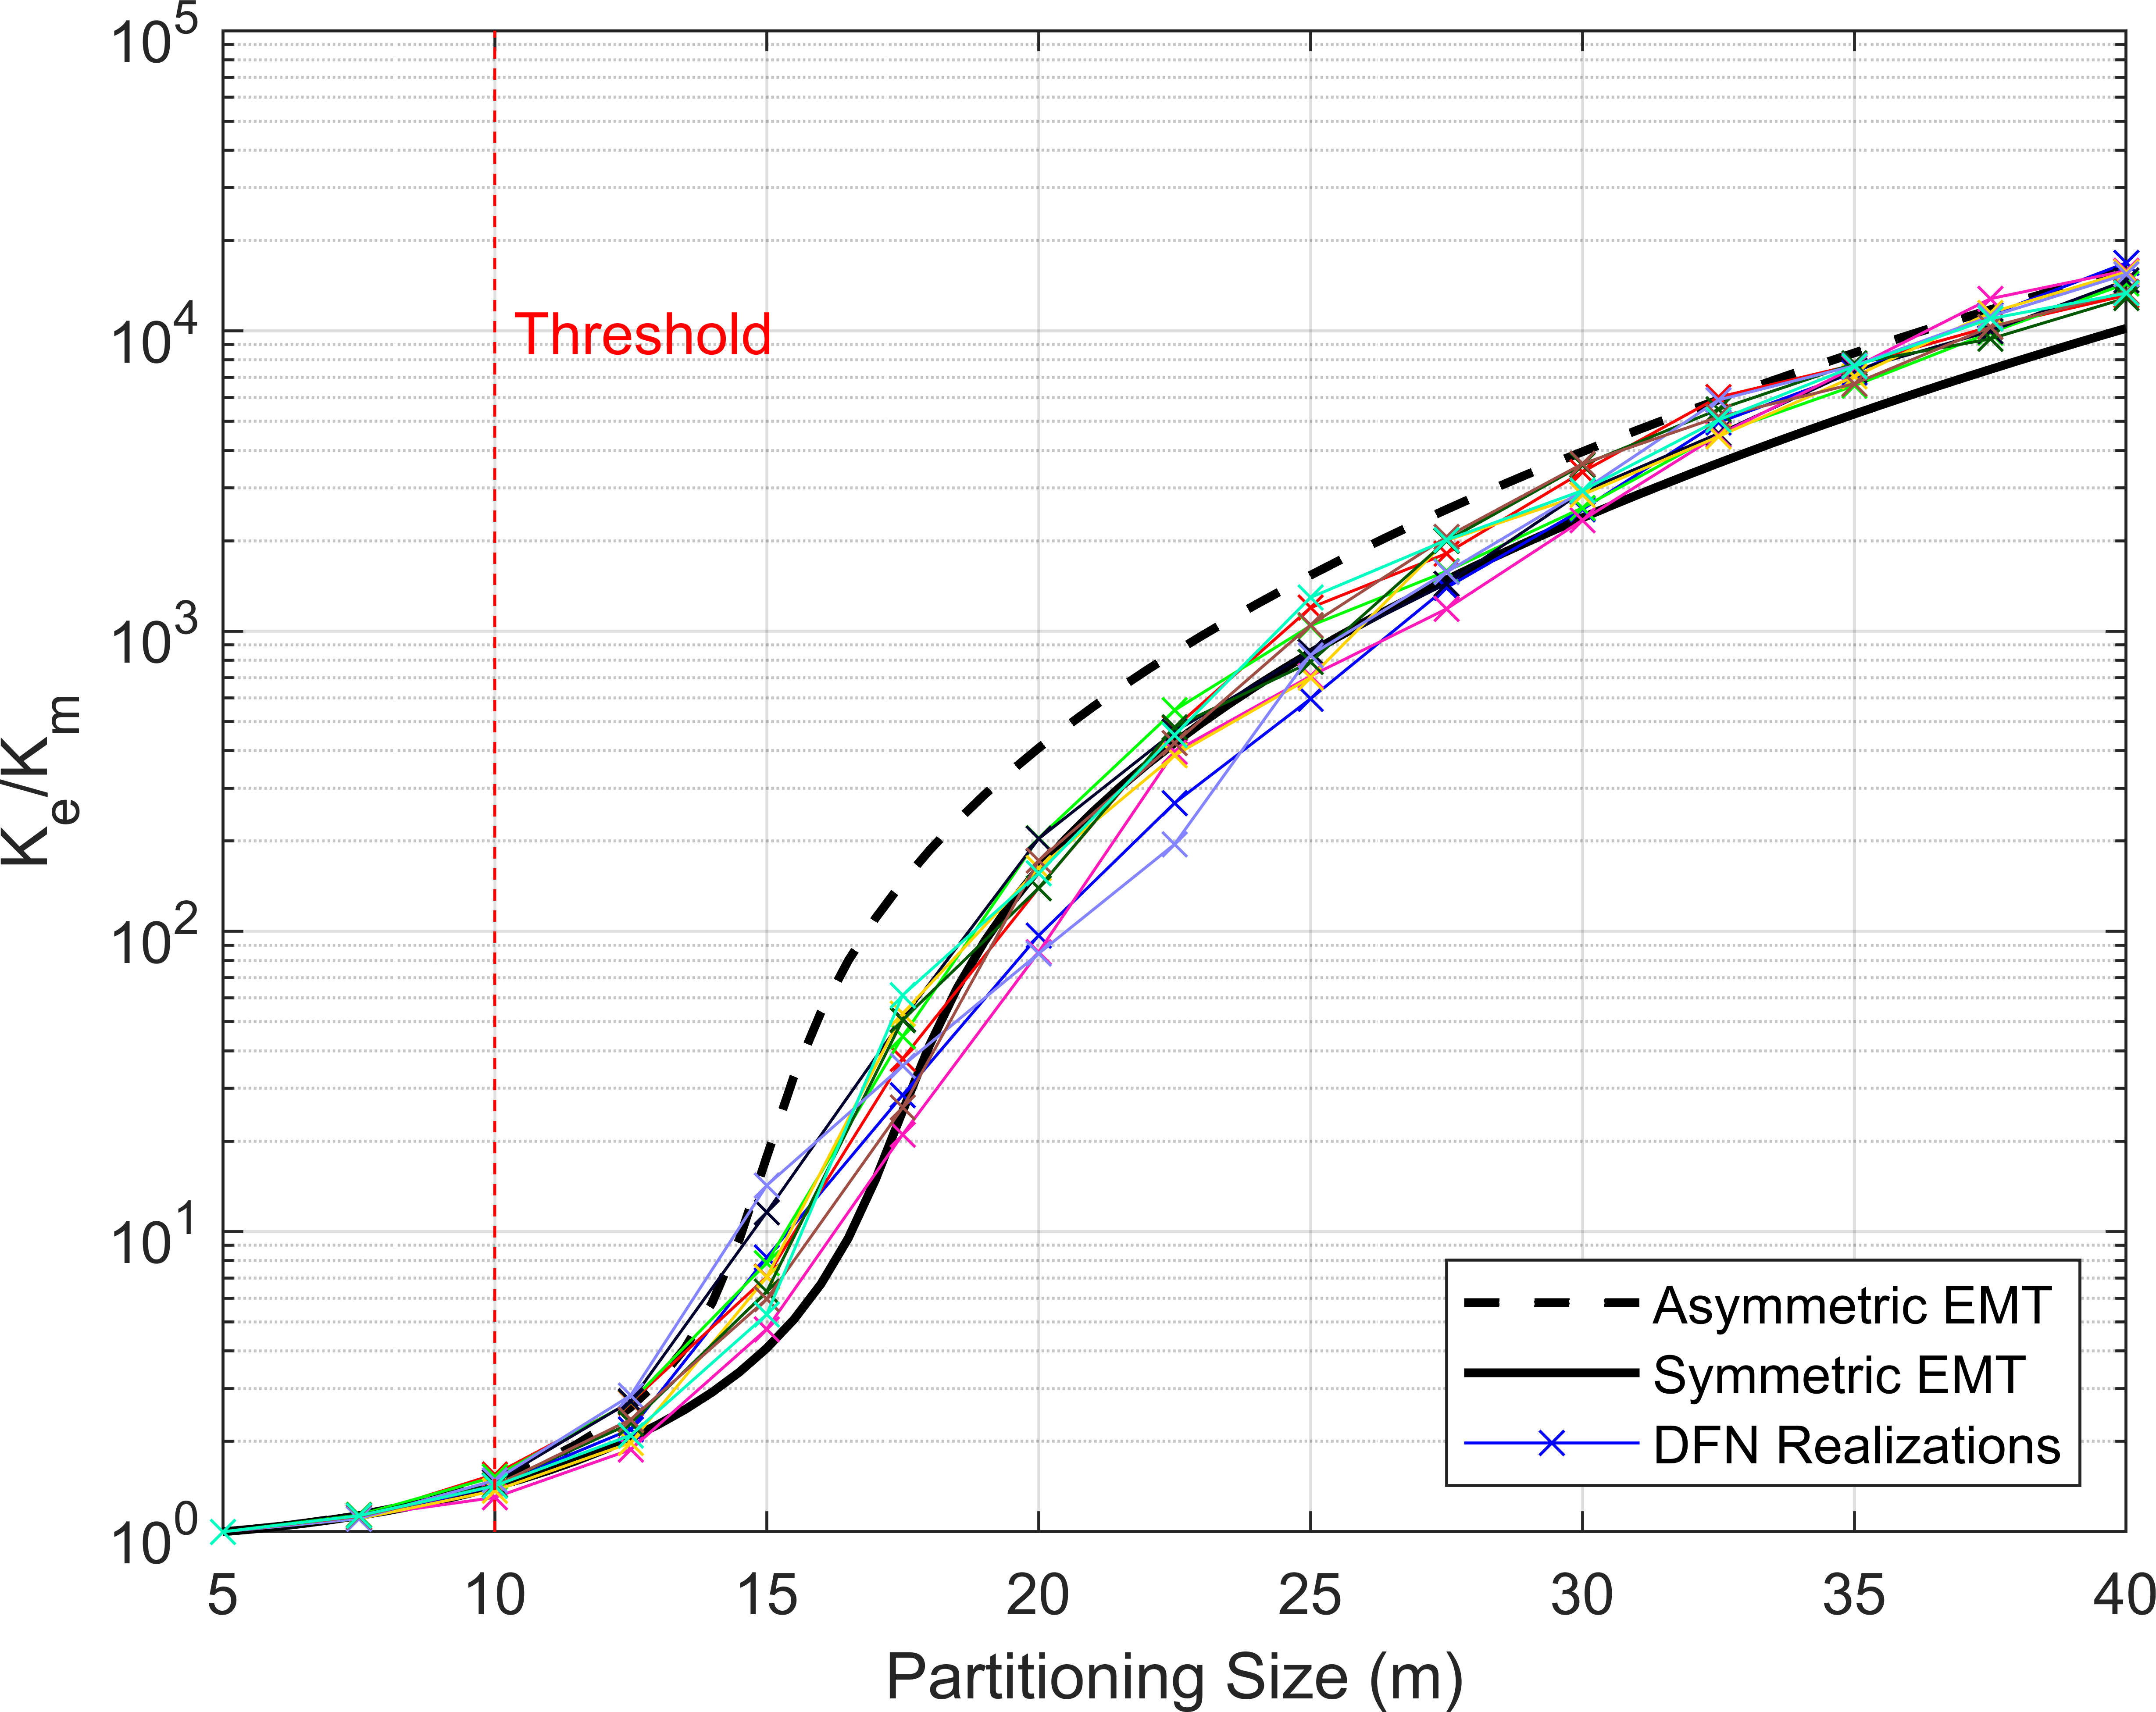
\includegraphics[width=\textwidth]{FSU/Plot_FSU_Case_09_nohead.png}
        \subcaption{Case 9}
        \label{fig:FSU_9}
    \end{subfigure}
    \\
    \begin{subfigure}{0.3\textwidth}
        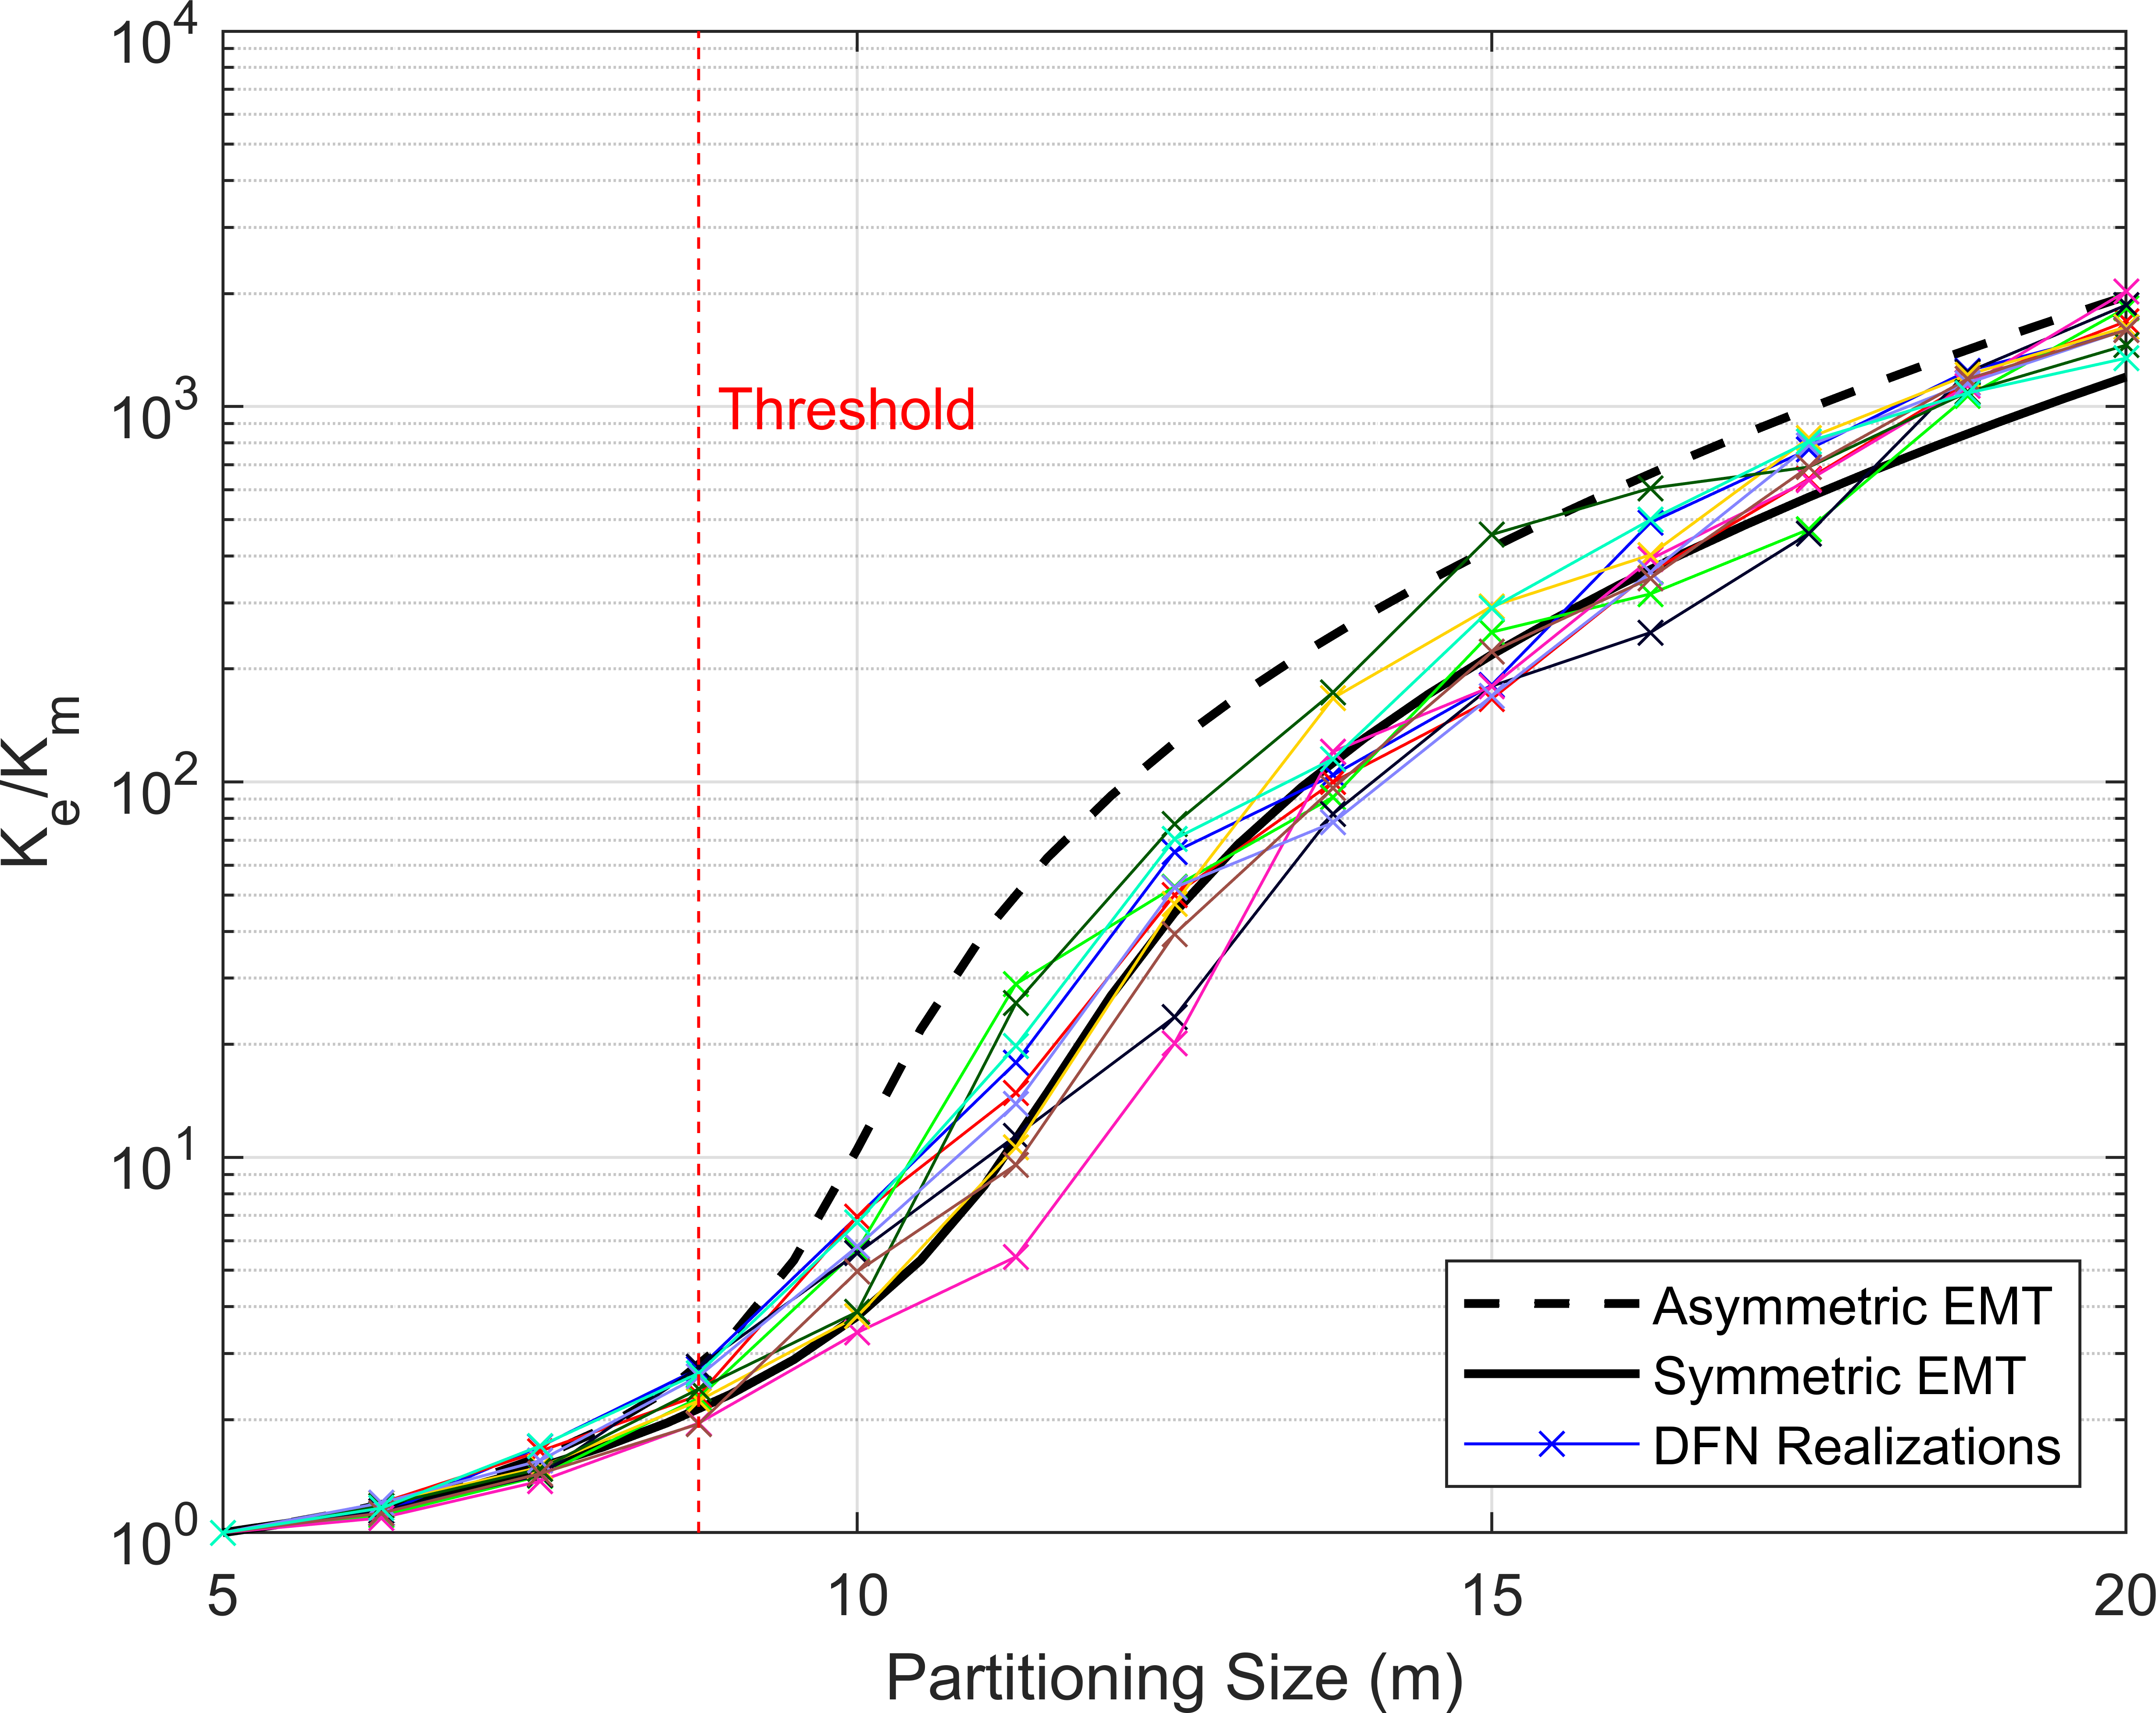
\includegraphics[width=\textwidth]{FSU/Plot_FSU_Case_10_nohead.png}
        \subcaption{Case 10}
        \label{fig:FSU_10}
    \end{subfigure}
    \begin{subfigure}{0.3\textwidth}
        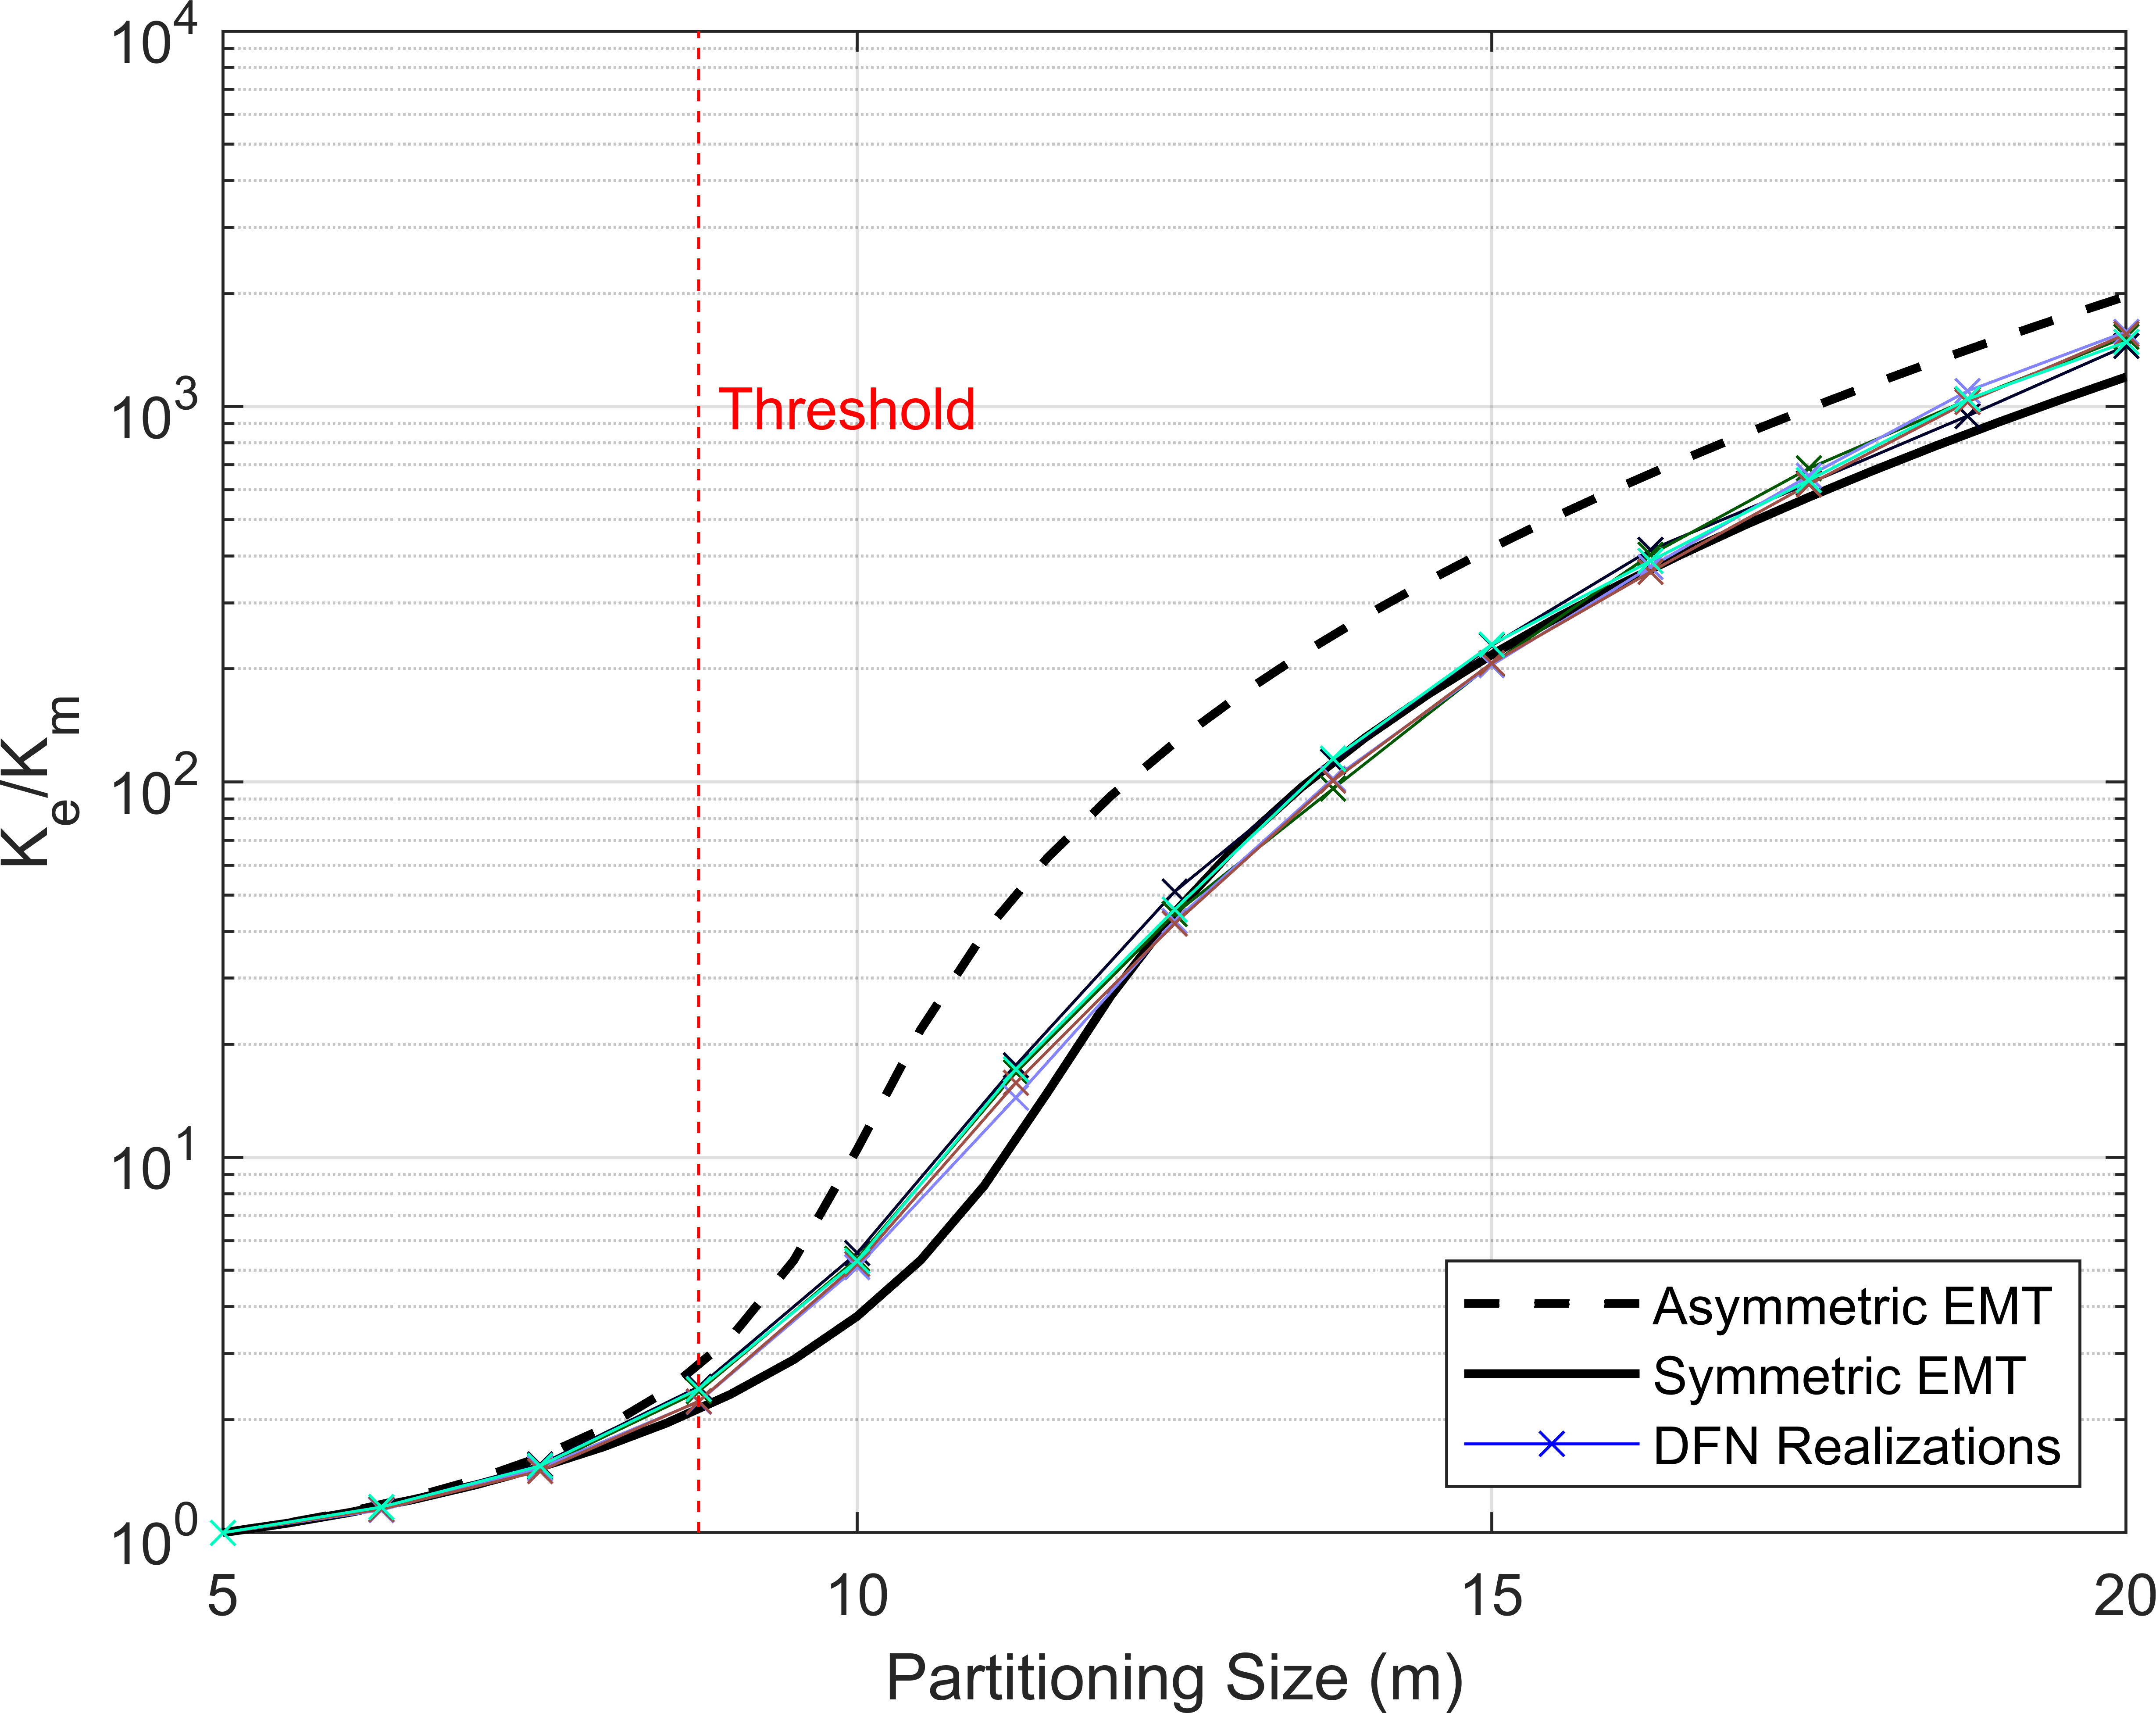
\includegraphics[width=\textwidth]{FSU/Plot_FSU_Case_11_nohead.png}
        \subcaption{Case 11}
        \label{fig:FSU_11}
    \end{subfigure}
    \begin{subfigure}{0.3\textwidth}
        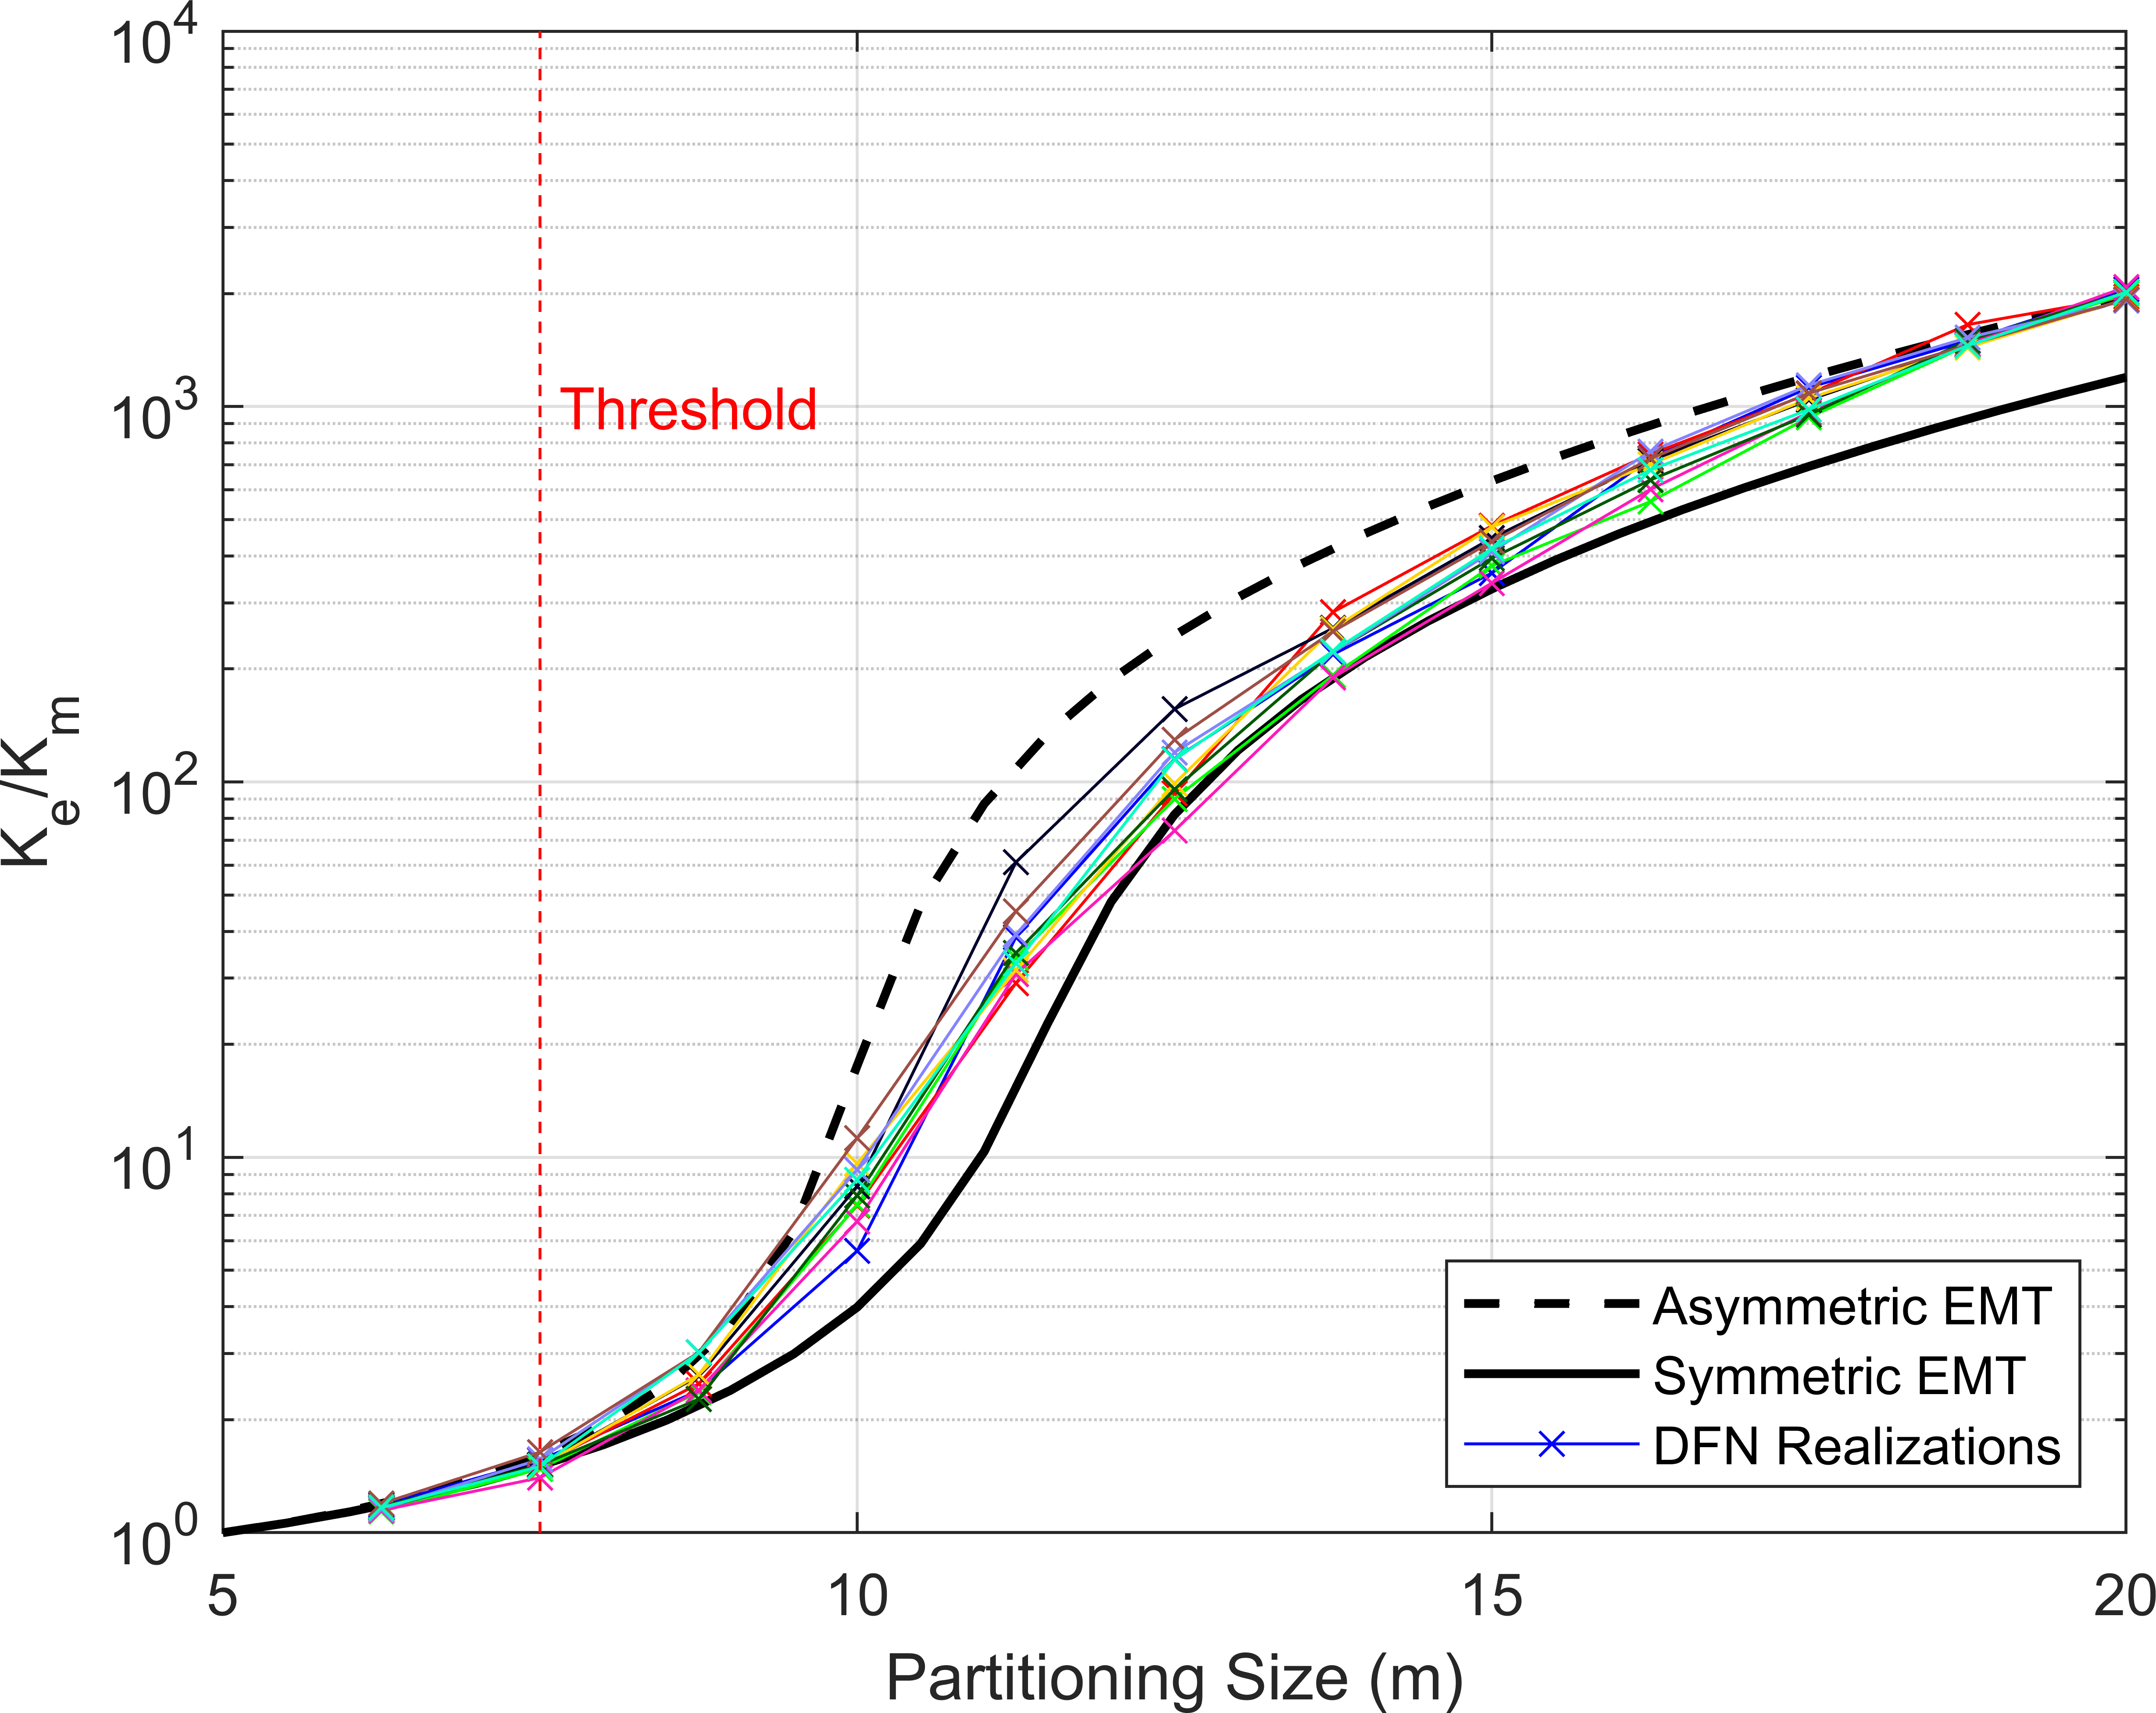
\includegraphics[width=\textwidth]{FSU/Plot_FSU_Case_12_nohead.png}
        \subcaption{Case 12}
        \label{fig:FSU_12}
    \end{subfigure}
    \\
    \begin{subfigure}{0.3\textwidth}
        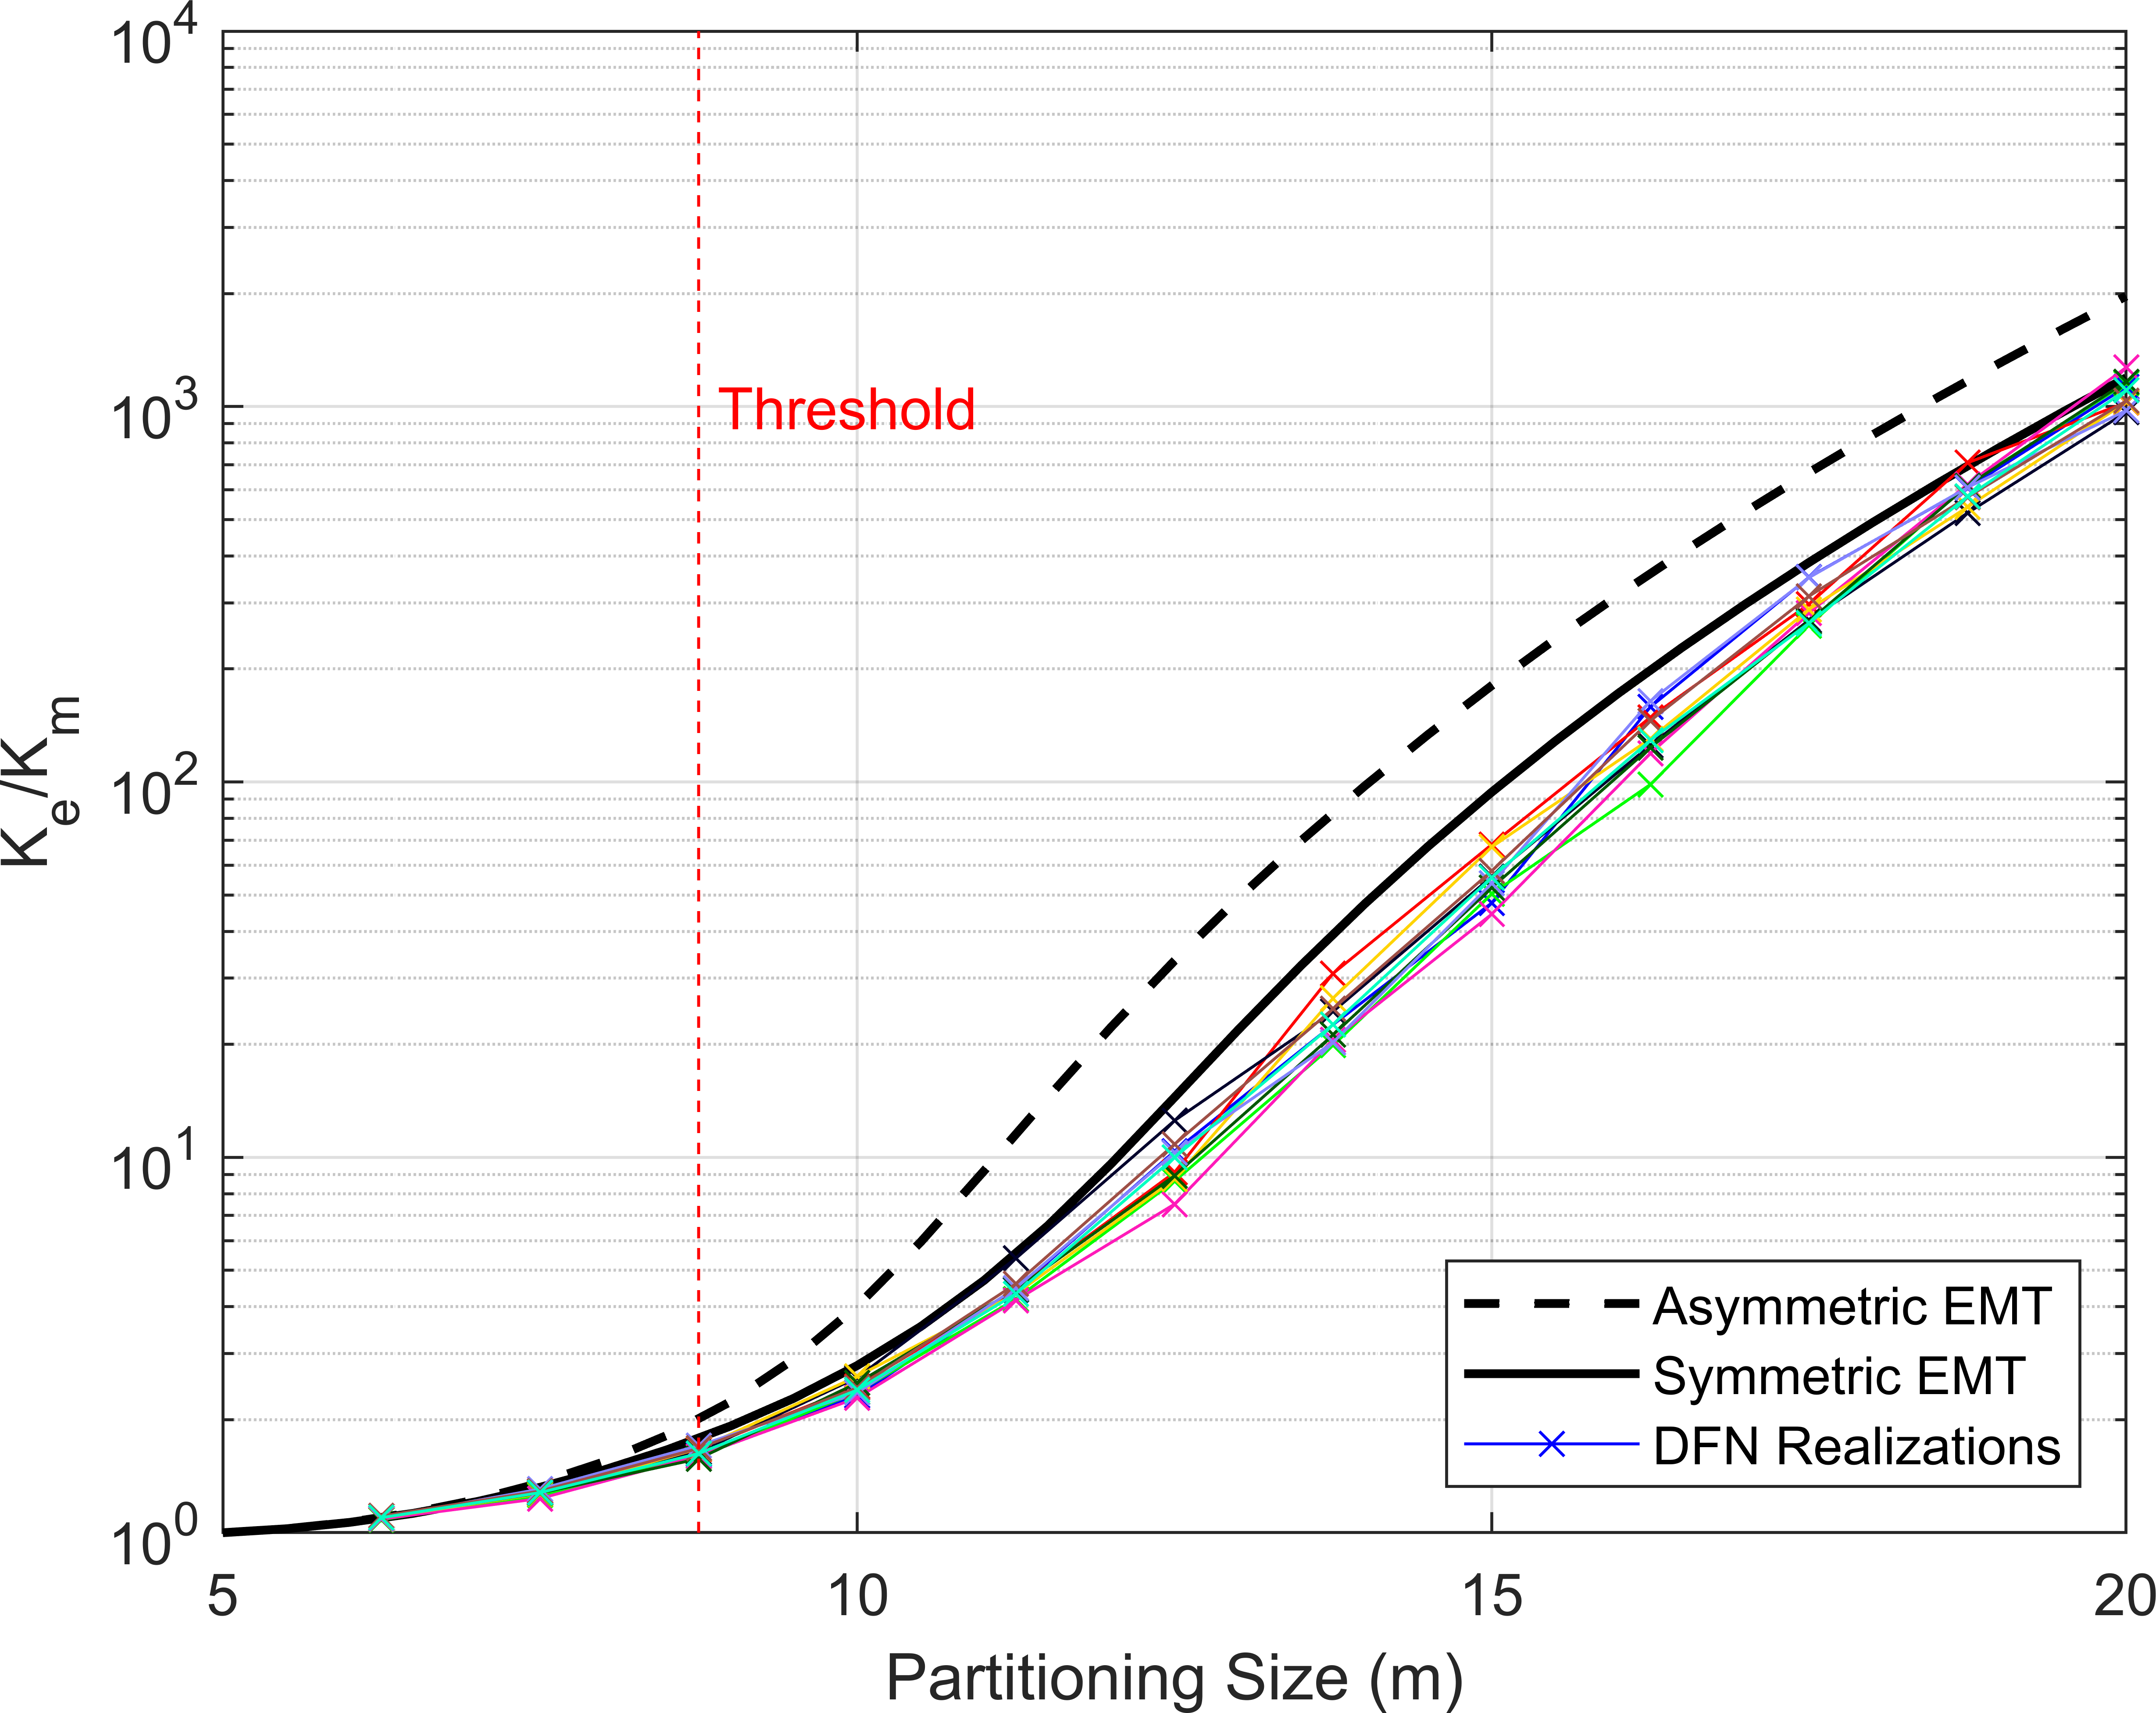
\includegraphics[width=\textwidth]{FSU/Plot_FSU_Case_13_nohead.png}
        \subcaption{Case 13}
        \label{fig:FSU_13}
    \end{subfigure}
    \begin{subfigure}{0.3\textwidth}
        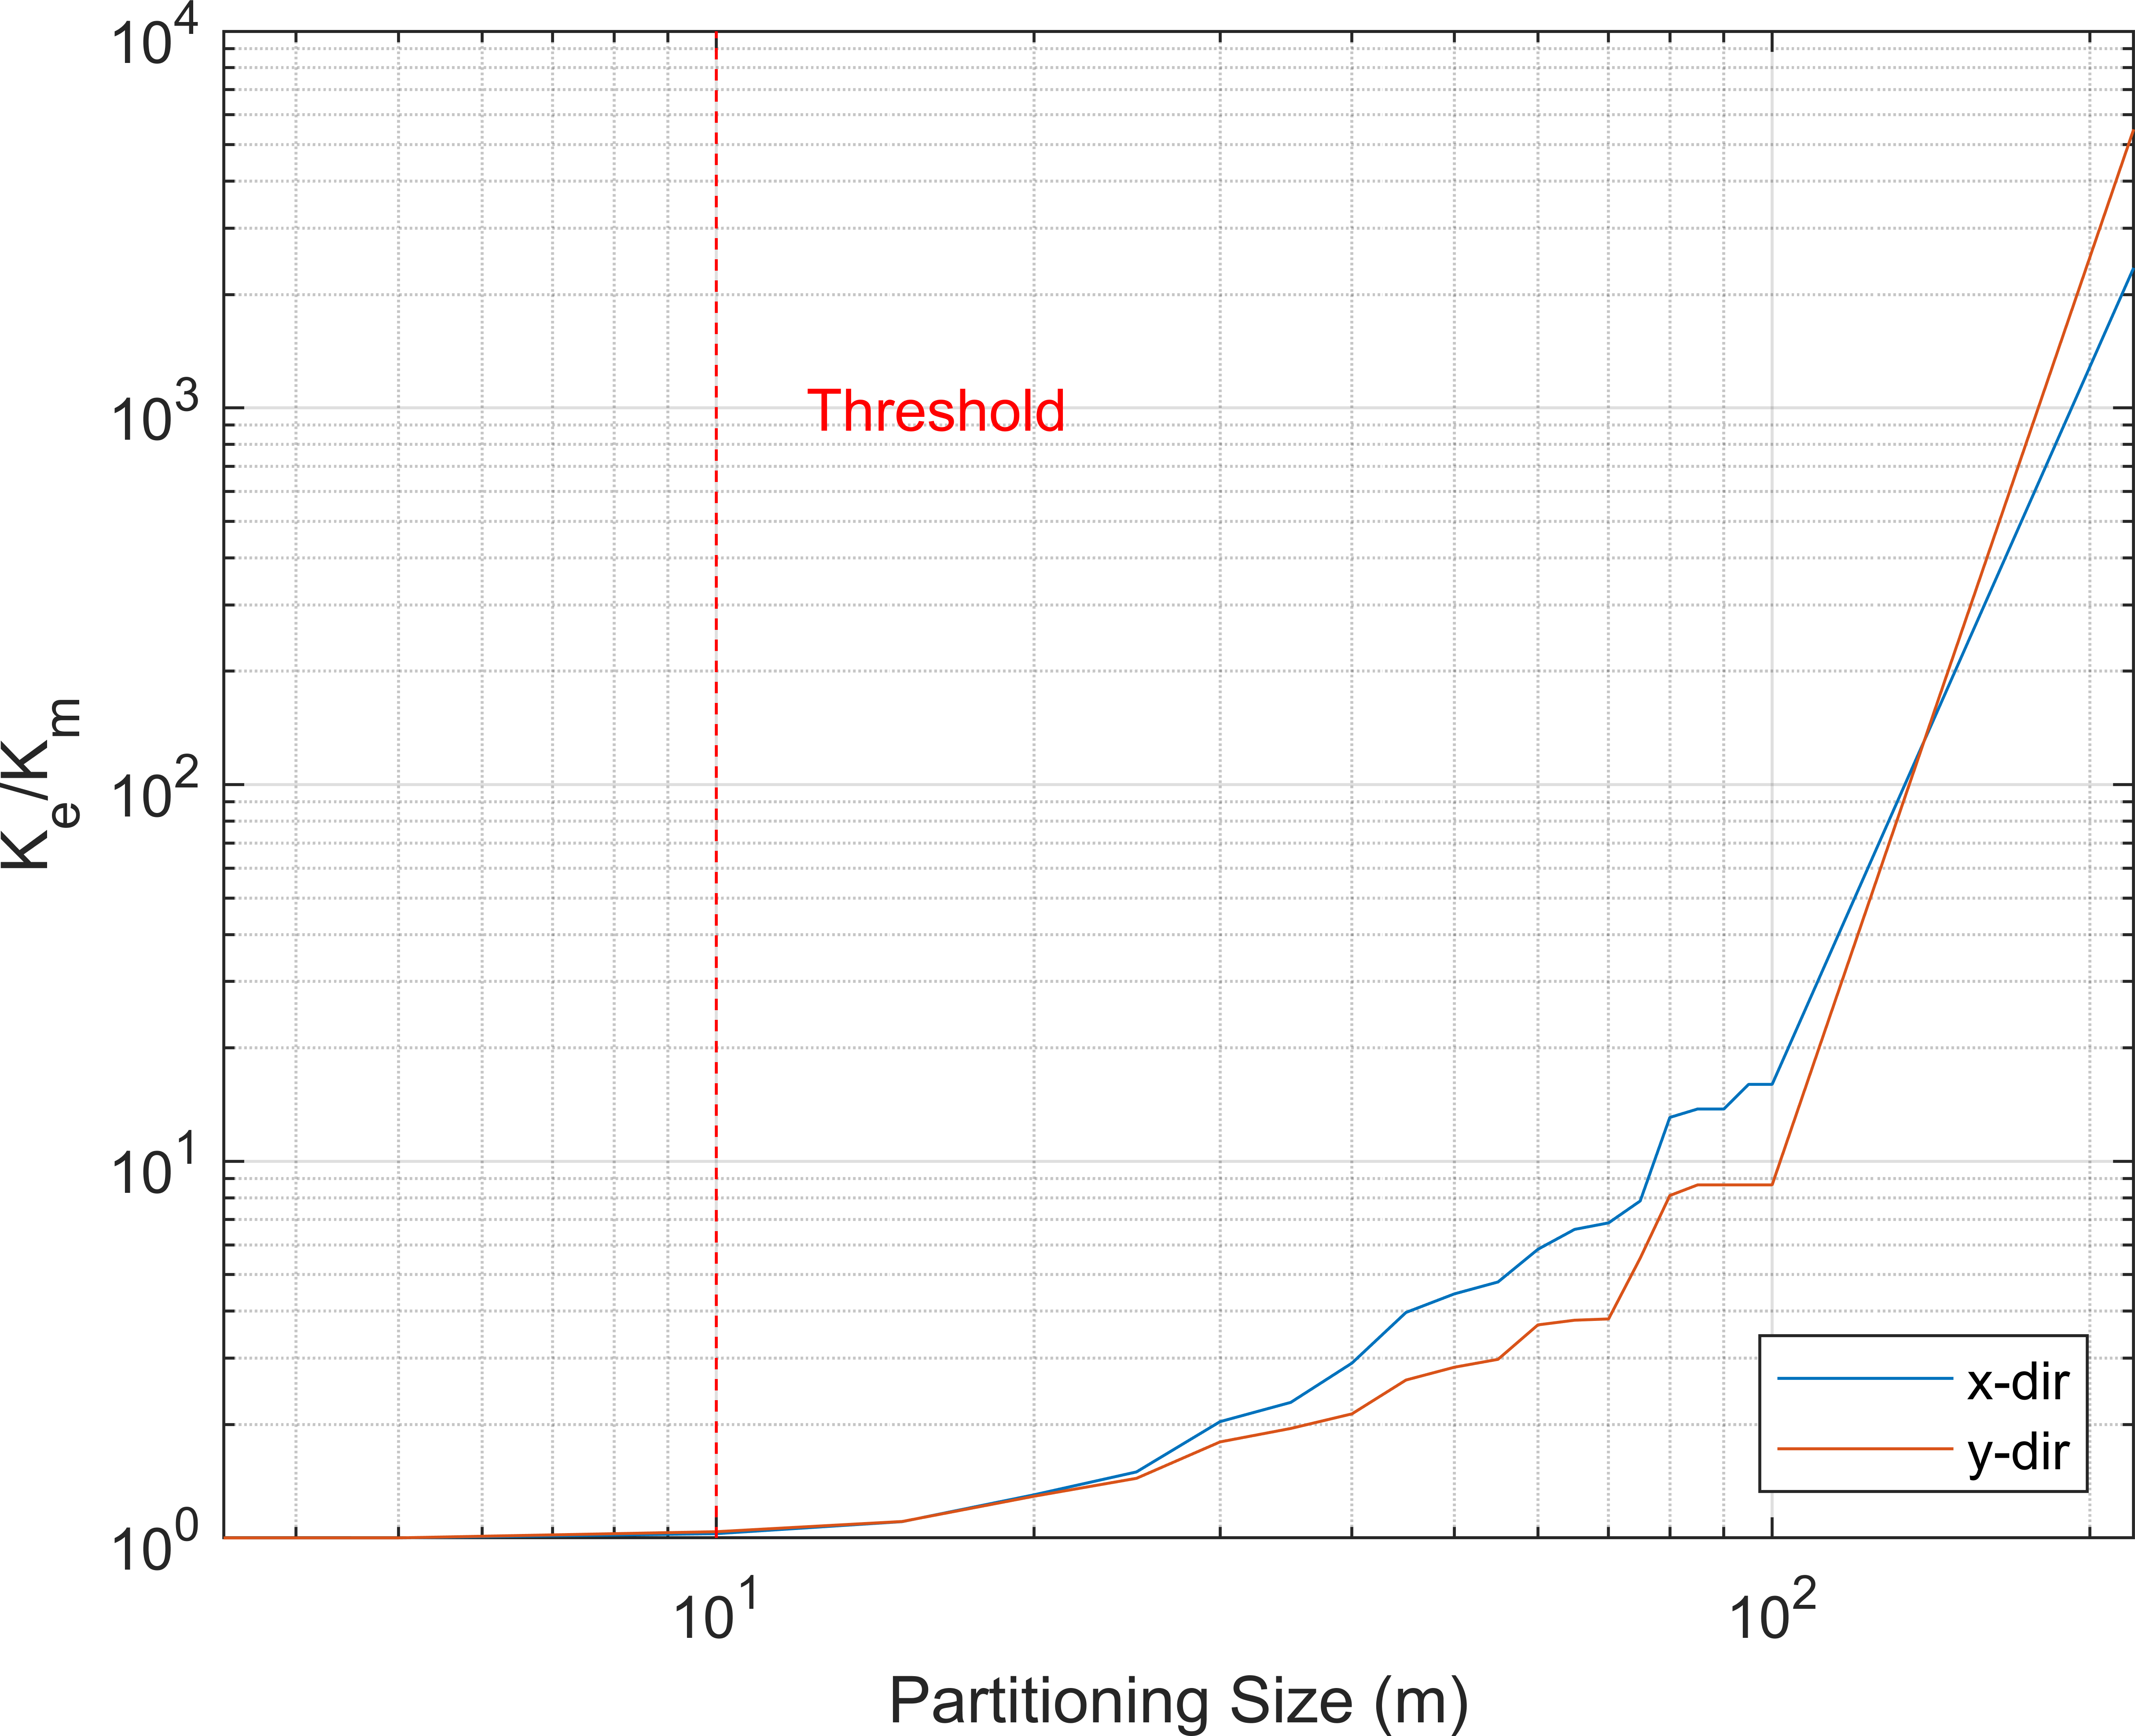
\includegraphics[width=\textwidth]{FSU/Apodi2_FSU_nohead.png}
        \subcaption{Apodi 2}
        \label{fig:FSU_Apodi_2}
    \end{subfigure}
    \begin{subfigure}{0.3\textwidth}
        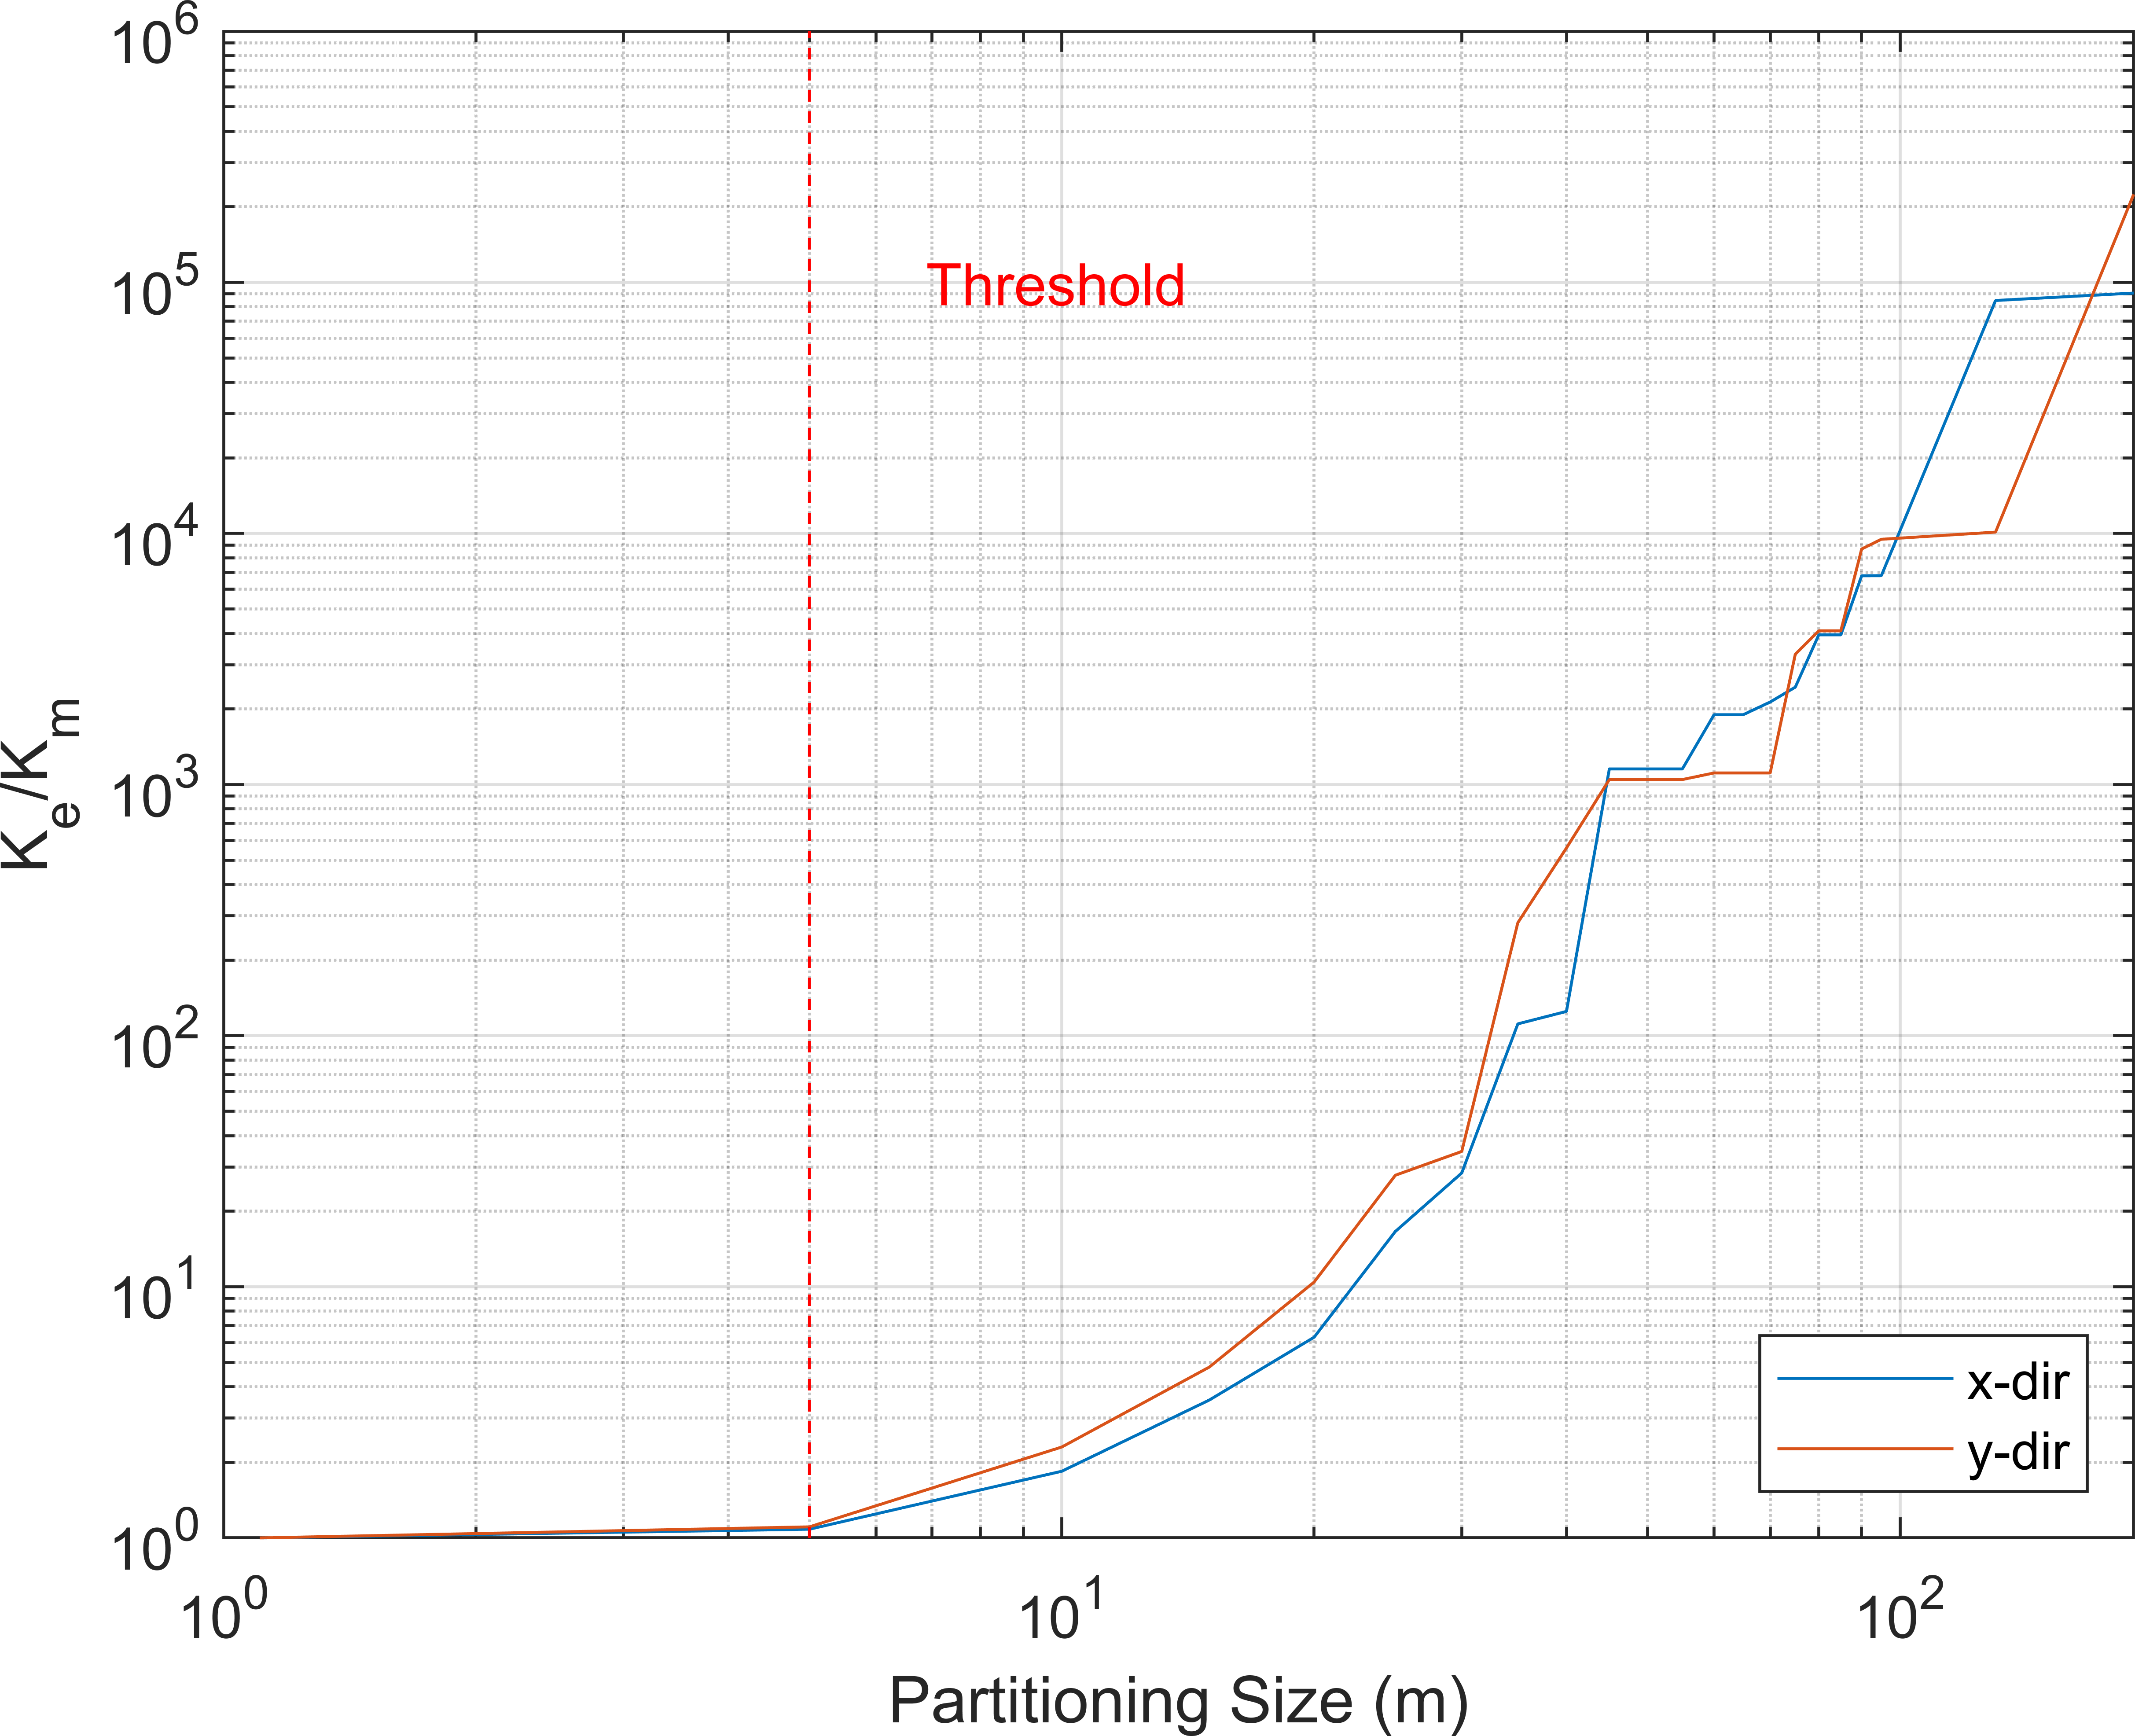
\includegraphics[width=\textwidth]{FSU/Apodi4_FSU_nohead.png}
        \subcaption{Apodi 4}
        \label{fig:FSU_Apodi_4}
    \end{subfigure}
    \caption{Fracture Subset Upscaling. (a)-(m) correspond to generated DFNs based on Table \ref{table:DFNparams}. (n)-(o) correspond to outcrop fracture data. Threshold partitioning sizes are identified from Figures \ref{fig:3D_DD} and \ref{fig:Apodi_DD}.}
    \label{fig:FSU}
\end{figure}
\end{document}